%-------------------------------------------------------------------------------------------
% Vorlage erstellt von sli92
% Latex für Einsteiger: http://latex.mschroeder.net/#textformatierung
% Formeln in Latex: http://www.hosi.de/latex/mathe.htm
%-------------------------------------------------------------------------------------------
%PRÄAMBEL
%-------------------------------------------------------------------------------------------

\documentclass[a4paper,14pt,headsepline]{scrartcl}

\usepackage[ngerman]{babel}
\usepackage[utf8]{inputenc}
\usepackage{fancyheadings}
\usepackage{graphicx}
\usepackage{eurosym}
\usepackage{setspace}

\usepackage{hyperref}

\usepackage{tabularx}
\newcolumntype{L}[1]{>{\raggedright\arraybackslash}p{#1}} % linksbündig mit Breitenangabe
\newcolumntype{C}[1]{>{\centering\arraybackslash}p{#1}} % zentriert mit Breitenangabe
\newcolumntype{R}[1]{>{\raggedleft\arraybackslash}p{#1}} % rechtsbündig mit Breitenangabe

% Absatzeinrückung
%++++++++++++++++++++++++++
%\setlength{\parskip}{5pt}
%\setlength{\parindent}{0pt}

\setlength{\parskip}{1.5em}
\setlength{\parindent}{0pt}

% Kopf- und Fußzeile
%++++++++++++++++++++++++++

\pagestyle{fancy}
\lhead{\bfseries netcon}
%\chead{Lipp}
\rhead{\nouppercase{\leftmark}}

%C für Center
\fancyfoot[C]{ \thepage}

%-------------------------------------------------------------------------------------------
%DOKUMENT
%-------------------------------------------------------------------------------------------

\begin{document}

% Titelseite
%++++++++++++++++++++++++++
\begin{titlepage}
    \begin{center}

\begin{center}
\textbf{HÖHERE TECHNISCHE BUNDESLEHRANSTALT WIEN 10 ABTEILUNG FÜR ELEKTRONIK}\\
 \vspace{2cm}
\LARGE\textbf{\textsc{DIPLOMARBEIT}}\\
     \vspace{2cm}
     
     

\includegraphics[width=0.35 \paperwidth]{./bilder/logo.png} \\
 \huge \textbf{\textsf{Ethernetbasiertes Messsystem}} \\
\vspace{1cm}
Verfasser \\
\vspace{0.5cm}
 \normalsize Sebastian Lipp \\
 Martin Pietryka \\
  
\vspace{1cm}
\huge Betreuer \\
\vspace{0.5cm}
 \normalsize Prof. Dipl.-Ing. Herbert Kern \\
 
 \end{center}
 
 \vspace{2cm}
 
\huge
 \begin{tabular}{L{5cm}R{10cm}l}
 
    	Jahrgang         & {Eingereicht} \\
	\normalsize
    	5AHELI, 2011/12 & {\normalsize Wien, am 25. Mai 2012} \\

\end{tabular}\\
  
\end{center}

\end{titlepage}

\newpage

\onehalfspacing

\section*{Erklärung}
Wir versichern,

dass wir die vorliegende Diplomarbeit selbstständig verfasst, andere als die angegebenen Quellen und Hilfsmittel nicht benutzt und wir auch uns sonst keiner unerlaubten Hilfe bedient haben, dass wir dieses Diplomarbeitsthema bisher weder im In- noch im Ausland in irgendeiner Form als Prüfungsarbeit vorgelegt haben. 

Wien, am 25. Mai 2012

\_\_\_\_\_\_\_\_\_\_\_\_\_\_\_\_\_\_\_\_\_\_\_\_   \newline Sebastian Lipp 

\_\_\_\_\_\_\_\_\_\_\_\_\_\_\_\_\_\_\_\_\_\_\_\_   \newline Martin Pietryka

\newpage

\section*{Zusammenfassung}
Das Ziel dieser Diplomarbeit war die Entwicklung eines flexiblen Messsystems auf Ethernet-Basis, zur einfachen Einbindung in vorhandene Netzwerkstrukturen und zugleich die Bereitstellung einfacher Werkzeuge für die Erstellung eines solchen Systems. Deshalb stehen alle Entwicklungen bzw. die gesamte Diplomarbeit unter OpenSource. Da die Ethernet-Schnittstelle mit TCP/IP kein Echtzeitverhalten garantiert, wurde das System nur für zeitunkritische Aufgaben ausgelegt. 

\textbf{Hardware}

Es wurden netzwerkfähige Messmodule entwickelt, die das von uns festgelegte Protokoll implementieren und Werkzeuge geschaffen für die Erstellung eigener Messmodule. Ein sogenannter UART-Umsetzer macht es sogar möglich eigene Messmodule um Netzwerkfähigkeit zu erweitern. 

\textbf{Software}

Eine eigens entwickelte Software für die Verwaltung der Module stellt die Schnittstelle für andere Applikationen, wie Websites und Smartphone-Apps bereit. Als Beispiel wurde eine einfache Website geschaffen, die alle im Netzwerk befindlichen Module und deren Messwerte anzeigt. 

\newpage

\section*{Abstract}
The aim of this diploma project was the development of a flexible measuring system for easily integrating in existing Ethernet networks and to provide simple tools for creating such a system. Therefore all developments - every code line - are OpenSource. Due to the fact that the Ethernet interface and TCP/IP don't support real-time behaviour this system isn't constructed for time critical tasks. 

\textbf{Hardware}

Network-compatible measuring modules were developed which implements our protocols and tools were built for creating own measuring modules. A so-called UART-Converter also makes it possible to extend network-compatibility to existing modules. 

\textbf{Software}

A specially developed software for managing the modules provides the interface to other applications like websites and smartphone-apps. For instance a simple website was built to list all modules and measured values.


\newpage

\section*{Vorwort}
Sie wollen Umweltgrößen an mehreren Standorten (aus der Ferne) überwachen? An den Standorten ist lediglich ein gemeinsames Ethernet-Netzwerk verfügbar und für den Aufbau eines eigenen Netzes fehlt das Budget?

Im Rahmen dieser Diplomarbeit, wurde mit \textbf{netcon} ein quelloffenes, flexibles Messsystem auf Ethernet-Basis geschaffen. Dabei wurde darauf Rücksicht genommen, erfahrene Endanwender, Unternehmen und Entwickler gleichermaßen zu bedienen. Je nach Anwendungsfall und Vorkenntnissen sollten Sie in der Lage sein ihr eigenes Messsystem aufzubauen. 

Im ersten Kapitel folgt ein Überblick über die \textbf{allgemeine Konzeption} - Systemvoraussetzungen, Aufbau und Schnittstellen. Ein zweites Kapitel gibt eine Einführung in \textbf{grundlegende Begriffe}, die für ein tieferes Verständnis der Entwicklungen erforderlich sind. Danach folgt das große Kapitel, \textbf{Hardware}, das den Aufbau und die Funktionsweise der Messmodule behandelt, sowie in die genaue Verwendung der Schnittstellen und Protokolle auf der Hardwareseite einführt. Das letzte Kapitel, \textbf{Software}, beschreibt die Verwaltungsschicht und deren Interfaces für die Anzeige der Moduldaten.

Die beliegende CD enthält die Diplomarbeit als PDF, sowie den gesamten Quellcode des netcon-Systems in den Verzeichnissen netcon Module und netcon Software. 

\newpage

\section*{Danksagung}
Zuallererst bedanken wir uns bei unserem Betreuer, Prof. Dipl.-Ing. Herbert Kern, der diese Diplomarbeit überhaupt erst ermöglichte. Vielen Dank, dass Sie uns mit vielen tollen Ratschlägen zur Seite standen und irgendwie ein System in die Sache brachten.

Zudem möchten wir jedem danken, der uns Material für die Entwicklung unseres Messsystems zur Verfügung gestellt hat.

Und zuletzt vielen Dank an Matthias Subik, für viele tolle Tipps, die uns immer mal wieder aus dem Licht der Verzweiflung führten.

Vielen Dank! 


\newpage


\newpage

% Inhaltsverzeichnis
%++++++++++++++++++++++++++
\tableofcontents
\newpage

%Inhalt
%++++++++++++++++++++++++++

\section{Überblick [Lipp]}

Netcon ist zum einen ein Messsystem zur Einbindung in ein bestehendes Ethernet-Netzwerk, zum anderen aber auch das Ziel flexible Werkzeuge für die Erstellung eines solchen Systems bereitzustellen. Dabei stehen alle Entwicklungen unter OpenSource.

Da das System als Übertragungsmedium die Ethernet-Schnittstelle mit der TCP/IP-Protokollschicht verwendet, ist Echtzeitverhalten nicht garantiert. Dadurch ist es nur für zeitunkritische Aufgaben geeignet. 

\subsection{Zielgruppen}
Erfahrene Endandwender, genauso Entwickler sollten mit netcon in der Lage sein, ein Messsystem zu realisieren. Es wurden hardware- und softwareseitig einfache Schnittstellen geschaffen um je nach Wunsch und vorherrschenden Kenntnissen eigene Anwendungen zu erstellen. 

Der Anwender kann sich entscheiden, entweder entwickelt er auf Basis der Spezifikationen die netzwerkfähigen Module selbst, oder aber er verwendet die im Rahmen dieser Diplomarbeit gewählten Mikrocontroller-Systeme. Dazu stellt netcon die entwickelte Firmware zur Verfügung. Weiters besteht für netzwerktechnisch unerfahrene Entwickler die Möglichkeit, ihre Module netzwerkfähig zu machen.
\newpage

Auch auf der Softwareseite stehen mehrere Wege offen. Entwickler können eigene Applikationen über die Schnittstelle der Verwaltungsschicht aufsetzen, oder aber auch die entwickelte Weboberfläche zur Anzeige der Moduldaten verwenden.

\subsection{Anwendungsbeispiele}
Netcon sieht in seiner Spezifikation mehrere Typen von Messmodulen vor. Folgende Liste zeigt Anwendungen, die unter anderem mit diesem System verwirklicht werden können:
\begin{itemize}
	\item Spannungsmessung
	\item Temperaturmessung
	\item Zeitmessung
\end{itemize}

\newpage

\subsection{Systemvoraussetzungen}

Das netcon Messsystem wurde für dein Einsatz in einem Ethernet-Netzwerk konzipiert. Dieses muss zumindest über folgende Komponenten verfügen:
\begin{itemize}
	\item Anschlussmöglichkeiten für die Module (Router/Switch/WLAN)
	\item DHCP-Server für die IP-Adressvergabe
	\item \textbf{Server} - Javafähige Betriebsumgebung für die Verwaltungsschnittstelle z.B. PC, Embedded System
	\item \textbf{Client} - Anzeigegerät z.B. Smartphone, Computer
\end{itemize}

Zusätzlich wird gegebenenfalls ein PHP-fähiger Webserver benötigt, um die bereits entwickelte Website verwenden zu können. Die genauen Anforderungen an die Softwareumgebung, sowie die Einrichtung einer Java Runtimte Environment (JRE) und eines Webservers sind im Kapitel \textit{Software} nachzulesen.

Und nicht zu vergessen sind die wichtigsten Komponenten, die netzwerkfähigen Module. Diese können, wie bereits erwähnt, nach den netcon-Protokollen selbst entwickelt, oder aber auch nach Anleitung erstellt werden. Dazu mehr im nächsten Abschnitt.
\newpage

\subsection{Systemaufbau}
Im folgenden sind die zwei grundlegenden netcon-Komponenten inkl. ihrer Schnittstellen beschrieben. Je nachdem wie netcon genutzt werden soll, wird auf weitere Kapitel verwiesen.

\subsubsection{Module}
Die \textbf{Module} sind Hardware, die über Ethernet und TCP/IP erreichbar und abfragbar sind. 

\begin{figure}[h]
\begin{center}
\fbox{
	%Rahmengroesse	
	\begin{minipage}{0.7 \paperwidth}
	\begin{center}
	%Bildgroesse
	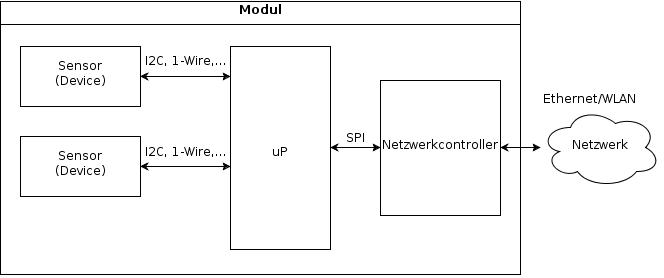
\includegraphics[width=0.5 \paperwidth]{./bilder/modul_aufbau.png}
	\caption{Aufbau eines Moduls}
	\label{modulaufbau}
	\end{center}
	\end{minipage}
}
\end{center}
\end{figure}

\newpage

Sie vereinen alle benötigten Komponenten - Mess- und Netzwerkeinheit - auf einer Platine (siehe Abb. \ref{modulaufbau}). Hier erfolgt die Übertragung zwischen den Sensoren und dem Mikroprozessor (uP) meist über Schnittstellen, wie I2C oder 1-Wire, während der Netzwerkcontroller per SPI mit dem uP kommuniziert. Über TCP und mit den beiden Protokollen \textit{netfind} und \textit{netcon} erfolgt die Abfrage durch den plattformunabhängigen Verwaltungs-Deamon \textit{netcond}. 

\textbf{Messmodule} umfassen beispielsweise Sensoren für Temperatur, Luftdruck und Zeit. Jeder dieser Sensoren wird von netcon als \textbf{Device} bezeichnet und kann mit seiner ID abgefragt werden.

Um den Modulen automatisch eine IP-Adresse zuweisen zu können und damit Konfigurationsarbeit zu ersparen, sollten diese auch das DHCP-Protokoll unterstützen.

Es bestehen grundsätzlich drei Möglichkeiten zur Erstellung von Modulen. Wenn Sie alle erforderlichen Kenntnisse besitzen, um die gesamte Entwicklung selbst zu übernehmen, informieren Sie sich im Kapitel \textit{Hardware} über den Aufbau der netcon-Protokolle. Sind Sie in der Lage einfache Messmodule ohne Netzwerkfähigkeit zu erstellen, verbinden Sie doch ein zusätzliches Netzwerkmodul (siehe Abb. \ref{modulaufbau2}). Diese Möglichkeit erfordert lediglich die Implementierung der Seriellen Schnittstelle (UART). Genauso können die im Rahmen dieser Diplomarbeit konzpierten Module mit ihrer Firmware für die Erstellung eigener Module herangezogen werden. Egal welche Wahl Sie treffen, das Kapitel \textbf{Hardware} unterstützt Sie in allen drei Fällen.

\begin{figure}[h]
\begin{center}
\fbox{
	%Rahmengroesse	
	\begin{minipage}{0.8 \paperwidth}
	\begin{center}
	%Bildgroesse
	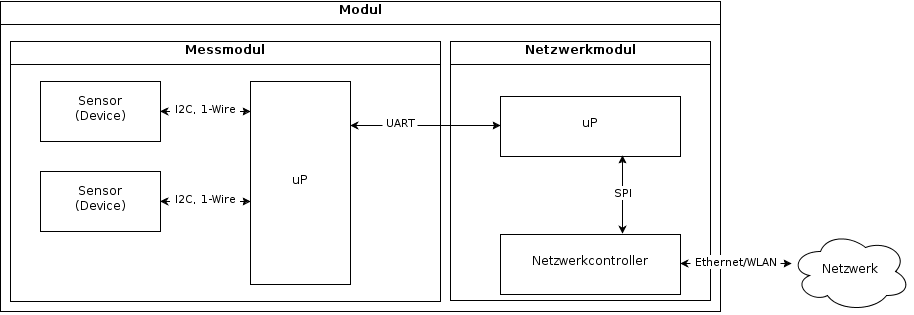
\includegraphics[width=0.7 \paperwidth]{./bilder/modul_aufbau2.png}
	\caption{Netzwerkfähiges Messmodul mittels LAN-UART Umsetzer}
	\label{modulaufbau2}
	\end{center}
	\end{minipage}
}
\end{center}
\end{figure}

\newpage

\subsubsection{Software}
Die Verwaltungsschnittstelle \textbf{netcond} ist eine in Java geschriebene Hintergrundanwendung (Daemon), die sich um die Verwaltung der Module kümmert. Wie in Abb. \ref{netcond} erkennbar können über das netcon Application Interface (netcon API) per TCP die Moduldaten abgefragt werden. Die Anwendung kann beispielsweise eine Website auf einem Webserver oder ein Smartphone-App sein. 

\begin{figure}[h]
\begin{center}
\fbox{
	%Rahmengroesse	
	\begin{minipage}{0.7 \paperwidth}
	\begin{center}
	%Bildgroesse
	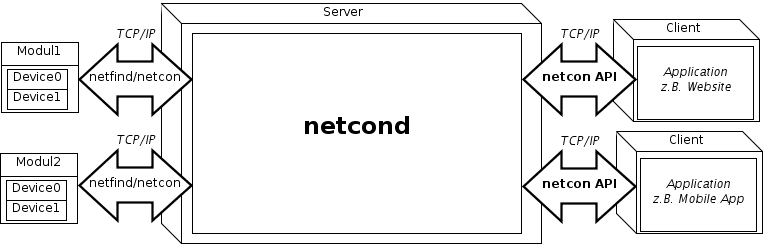
\includegraphics[width=0.7 \paperwidth]{./bilder/netcond.png}
	\caption{netcond}
	\label{netcond}
	\end{center}
	\end{minipage}
}
\end{center}
\end{figure}

\newpage
Soll die Anwendung zur Anzeige der Messdaten selbst entwickelt werden, führt das Kapitel \textbf{Software} in die Verwendung der Softwareschnittstelle ein. Sonst kann die bereits entwickelte Website \textbf{netcon web} (siehe Abb. \ref{website}) verwendet werden. Dazu ist zusätzlich zur JRE ein http-Webserver mit PHP-Unterstützung erforderlich. Deren Installation und Konfiguration ist auch im Kapitel \textit{Software} erklärt. 

\begin{figure}[h]
\begin{center}
\fbox{
	%Rahmengroesse	
	\begin{minipage}{0.7 \paperwidth}
	\begin{center}
	%Bildgroesse
	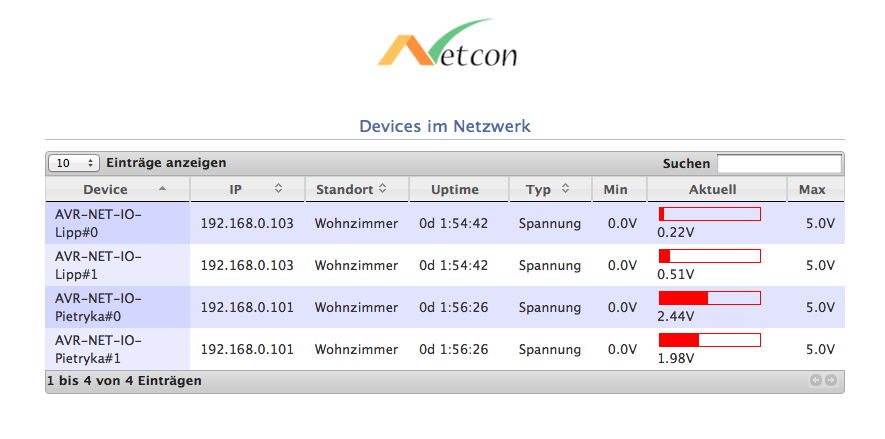
\includegraphics[width=0.7 \paperwidth]{./bilder/website.png}
	\caption{netcon web}
	\label{website}
	\end{center}
	\end{minipage}
}
\end{center}
\end{figure}

\newpage

\section{Grundlagen [Pietryka]}
\subsection{Network Byte Order}
In der Geschichte der Prozessoren und Heimcomputer gab es verschiedene Prozessorarchitekturen, diese verwendeten auch eine unterschiedliche Anordnung der Zahlen (welche auch aus mehr als einem Byte bestehen) im Speicher. Bei  der Kommunikation über das Netzwerk sollten die Zahlen aber immer die gleiche Bedeutung haben. Deshalb hat man sich bei Daten über das Netzwerk auf die sogenannten Network-Byte-Order geeinigt, diese wird auch als Big-Endian-Format bezeichnet, dabei werden die höherwertigen Bytes zuerst im Speicher gespeichert, also einer niedrigeren Adresse, bei der Netzwerkübertragung werden diese höherwertigen Bytes als erstes übertragen. Ein TCP/IP-Stack wie der uIP-Stack bietet verschiedene Funktionen um die der Host-Byte-Order, also die Byte-Order des Gerätes, in die Network-Byte-Order umzurechnen, sowie umgekehrt. Die Funktionen lauten:
\begin{quote}
\begin{verbatim}
Für 16 Bit Zahlen:
    Host to Network Byte Order:
        uint16_t htons(uint16_t i);
    Network to Host Byte Order:
        uint16_t ntohs(uint16_t i);

Für 32 Bit Zahlen:
    uint32_t htonl(uint32_t i);
    uint32_t ntohl(uint32_t i);
\end{verbatim}
\end{quote}

\subsection{OSI-Schichtenmodell}
Das OSI-Schichtenmodell ist ein von der ISO im Jahre 1983 standardisiertes Modell, welches als Designgrundlage für Kommunikationsprotokolle in Computernetzen dient. Dabei wird die Kommunikation beim OSI-Modell auf sieben Schichten bzw. Layern aufgeteilt. Für jede dieser Schichten sind Anforderungen und Aufgaben definiert, welche von entsprechenden Protokollen realisiert werden müssen. Eine konkrete Umsetzung ist aber nicht vorgegeben, daher gibt es für eine Schicht auch mehrere in Frage kommenden Protokolle.

\subsubsection*{Schicht 1: Bitübertragungsschicht}
Protokolle auf dieser Schicht kümmern sich darum, wie die unterschiedlichen Netzwerkgeräte untereinander verbunden sind, sowie welches Medium dafür verwendet wird. Hier geht es um die Übertragung einzelner Bits, es müssen je nach Übertragungsmedium verschiedene Codes oder Modulationsverfahren für die Übertragung von einzelnen Bits festgelegt werden. Weiterhin sind Geräte wie Antennen, Verstärker, Stecker und Buchsen ebenfalls auf dieser Schicht definiert.

Protokolle und Normen: V.24, V.28, X.21, RS 232, RS 422, RS 423, RS 499

\newpage

\subsubsection*{Schicht 2: Sicherungsschicht}
Auf dieser Schicht definierte Protokolle sollen sich darum kümmern, dass die Daten zuverlässig, im Sinne von fehlerfrei, ankommen. Dazu wird der Bitstrom in Blöcke (auch Frames genannt) unterteilt, diese Frames werden mit einer Prüfsumme versehen, welches es dem Empfänger erlaubt Fehler zu erkennen und ja nach Protokoll auch Fehler bis zu einem gewissen Grad zu korrigieren. Ein erneutes Anfordern von verworfenen Blöcken, oder das Erkennen von überhaupt nicht angekommenen Blöcken ist auf dieser Schicht nicht vorgesehen. Weiterhin wird im Protokoll eine sogenannte Zugriffskontrolle definiert, diese regelt, wann und wer auf das Medium zugreifen darf. Hardwareelemente auf dieser Schicht sind die Bridge und der Switch.

Bekannte Protokolle auf dieser Schicht sind das Ethernet-Protokoll, welches besser als das kabelgebundene lokale Netzwerk bekannt ist, oder das IEEE 802.11 Protokoll, welches das bekannte Wireless-LAN beschreibt.

\subsubsection*{Schicht 3: Vermittlungsschicht}
Diese Schicht kümmert sich um das Weiterleiten von Paketen bei paketorientierten Diensten. Meist besteht zwischen Sender und Empfänger keine direkte Verbindung, daher muss das Paket mehrere Zwischenstationen durchlaufen bis es an seinem Ziel ankommt. Dieser Vorgang wird Routing genannt, die entsprechende Hardware für diese Schicht ist der Router.

Protokolle und Normen: X.25, ISO 8208, ISO 8473 (CLNP), ISO 9542 (ESIS), IP, IPsec, ICMP

\subsubsection*{Schicht 4: Transportschicht}
Die Aufgabe dieser Schicht ist einerseits die Stauvermeidung, andererseits stellt diese Schicht mit ihren Protokollen für die höheren Schichten einen einheitlichen Zugriff bereit. Deswegen müssen die höheren Schichten auch nicht wissen welche Protokolle auf den unteren Schichten arbeiten. Bekannte Protokolle sind TCP, welches bereits die Datensicherheit durch Neuübertragungen vorgesehen hat, sowie UDP, welches, außer einer Prüfsumme, keine Sicherheitsmechanismen hat.

\subsubsection*{Schicht 5: Sitzungsschicht}
Die Sitzungsschicht sorgt für die Prozesskommunikation zwischen zwei Systemen, sie sorgt dafür, dass Zusammenbrüche einer Sitzung oder ähnliche Störungen behoben werden. Dazu werden sogenannte Wiederaufsetzpunkte eingeführt, an denen die Sitzung nach einem Ausfall der Verbindung wieder fortgesetzt werden kann.

\subsubsection*{Schicht 6: Darstellungsschicht}
Bei der Darstellungsschicht geht es darum, die systemabhängige Darstellung der Daten in eine unabhängige Form zu bringen. Diese erlaubt den korrekten Datenaustausch zwischen zwei unterschiedlichen Systemen. Ebenfalls zur Schicht 6 gehören Verschlüsselung und Datenkompression, sowie eventuell das Übersetzen zwischen verschiedenen Datenformaten.

\subsubsection*{Schicht 7: Anwendungsschicht}
Die oberste Schicht, die sogenannte Anwendunsschicht verschafft Anwendungen den Zugriff zum Netz. Hierzu zählen Alle Anwendungen die einem Netzwerkkommunikation Benötigen wie E-Mail Client, Browser, etc. Der Zugriff zum Netzwerk ist vollständig von der Hardware abstrahiert und geht über logische Verbindungen. Einige Protokolle auf dieser Schicht sind HTTP, FTP, SSH, Telnet, sowie jedes weitere Protokoll, welches Programme zum Austausch von Daten im Netzwerk verwenden. Bei dieser Diplomarbeit wurde hierzu zum Beispiel das netcon Protocol entwickelt, dieses ist ein Schicht 7 Protokoll.

\newpage 
\subsection{Ethernet}
Das Ethernet beschreibt unter anderem Protokolle sowie Hardware für ein kabelgebundenes Datennetz, es ist auch unter dem Namen Local-Area-Network (LAN) bekannt. Die Übertragungsraten sind mit 10Mb/s, 100Mb/s, 1Gb/s  und 10Gb/s spezifiziert. Das Ethernet Protokoll umfasst die OSI-Schichten 1 und 2, die Übertragung läuft in Paketen, den sogenannten Ethernet-Frames ab. Diese Frames haben eine minimale Länge von 64 Bytes und können Maximal 1518 Bytes groß werden. Sind die Nutzdaten kleiner als 46 Bytes so wird der Rest mit Nullen aufgefüllt um die minimale Größe von 64 Bytes zu erreichen.

\begin{figure}[h]
\begin{center}
\fbox{
	%Rahmengroesse	
	\begin{minipage}{0.7 \paperwidth}
	\begin{center}
	%Bildgroesse
	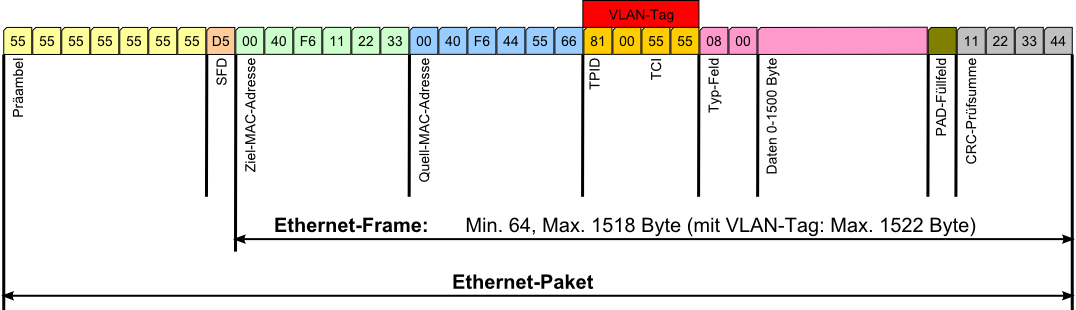
\includegraphics[width=0.7 \paperwidth]{./bilder/ethernetframe.png}
	\caption{Ethernetframe}
	\end{center}
	\end{minipage}
}
\end{center}
\end{figure}

Das Präambel sowie der Start-Frame-Delimiter (SFD) dienen dazu, um auf Bitebene einerseits den Beginn eines Ethernetframes zu erkennen, andererseits um eventuell eine Taktsynchronisation durchzuführen, da das Präambel ein alternierendes Bitmuster enthält. Danach kommt jeweils eine Ziel- sowie eine Quell-MAC-Adresse, diese Adressen sind jeweils 6 Bytes lang. Das VLAN-Tag ist optional und dient dazu, innerhalb eines physikalischen Ethernet-Netzwerks noch zwischen virtuellen (Virtual Local Area Network) Netzwerken unterscheiden zu können. Das Typ-Feld gibt an, welches Protokoll auf der nächsthöhrenen Schicht Verwendung findet, einige von denen sind:
\begin{itemize}
	\item \begin{verbatim}0x8000:    IP Version 4 \end{verbatim}
	\item \begin{verbatim}0x0806:    Address Resolution Protocol (ARP) \end{verbatim}
	\item \begin{verbatim}0x86DD:    IP Version 6 \end{verbatim}
\end{itemize}
Danach kommen die Nutzdaten, diese müssen mindestens eine Länge von 46 Bytes haben, ist dies nicht der Fall, so werden die restlichen Bytes mit Nullen, dem sogenannten Padding aufgefüllt, die maximale Länge der Nutzdaten beträgt 1500 Bytes. Die letzten 4 Bytes bilden eine sogenannte CRC-Prüfsumme, durch diese lässt sich berechnen ob alle Bytes im Ethernet-Frame korrekt übertragen wurden, ist dies nicht der Fall so sollte dieser Frame verworfen werden.

\subsubsection{MAC-Adresse}
Die MAC-Adresse (Media-Access-Control-Adresse) ist eine Adresse welche Netzwerkgeräte, genauer gesagt Netzwerkadapter, eindeutig identifiziert, Ethernet Pakete werden mithilfe dieser Adresse adressiert. Diese Adresse ist 48 Bit lang und ist auf der Welt eindeutig für jedes Netzwerkgerät. Die Schreibweise erfolgt in hexadezimaler Darstellung wie 00:80:41:AE:FD:7E oder 00-80-41-AE-FD-7E. Will man seine Netzwerkfähigen Geräte am Markt verkaufen, so benötigt man gültige MAC-Adressen, diese kann man in Blöcken kaufen. Kleinere Unternehmen können Blöcke mit 4096 MAC-Adressen kaufen, größere Unternehmen besitzen die Möglichkeit einen Block mit 16,8 Millionen Adressen zu kaufen.

Entwickelt man aber geringere Stückzahlen, so gibt es beispielsweise von der Firma Microchip bestimmte EEPROM Bausteine, welche mit einer bereits vorprogrammierten und natürlich gültigen MAC-Adresse geliefert werden. Eine weitere Möglichkeit gültige MAC-Adressen während der Entwicklung zu vergeben sind die sogenannten lokal administrierten Adressen, dabei wird im ersten Byte das zweite Bit auf 1 gesetzt. Ist dies der Fall, so handelt es sich um eine lokal administrierte Adresse, der Nachteil hierbei ist natürlich, dass diese Adresse nicht mehr eindeutig ist.

\subsubsection{Broadcast}
Bei einem sogenannten Broadcast wird im Ethernet-Header eine spezielle MAC-Adresse als Ziel angegeben, nämlich FF:FF:FF:FF:FF:FF, Pakete mit dieser Zieladresse werden an alle Geräte in einem LAN-Netzwerk verschickt, jedoch nicht in ein anderes Netzwerk geroutet.

\newpage
\subsection{IP}
Das Internet-Protocol stellt eine hardwareunabhängige Schicht für die höheren Schichten zur Verfügung, dabei erfolgt die Adressierung durch logische Adressen, die IP-Adressen. Diese Adressen sind 4 Bytes lang und werden in der Form XXX.XXX.XXX.XXX angeschrieben wobei natürlich jedes Byte von 0-255 geht. Ein IP-Paket hat den folgenden Aufbau:
\begin{figure}[h]
\begin{center}
\fbox{
	%Rahmengroesse	
	\begin{minipage}{0.7 \paperwidth}
	\begin{center}
	%Bildgroesse
	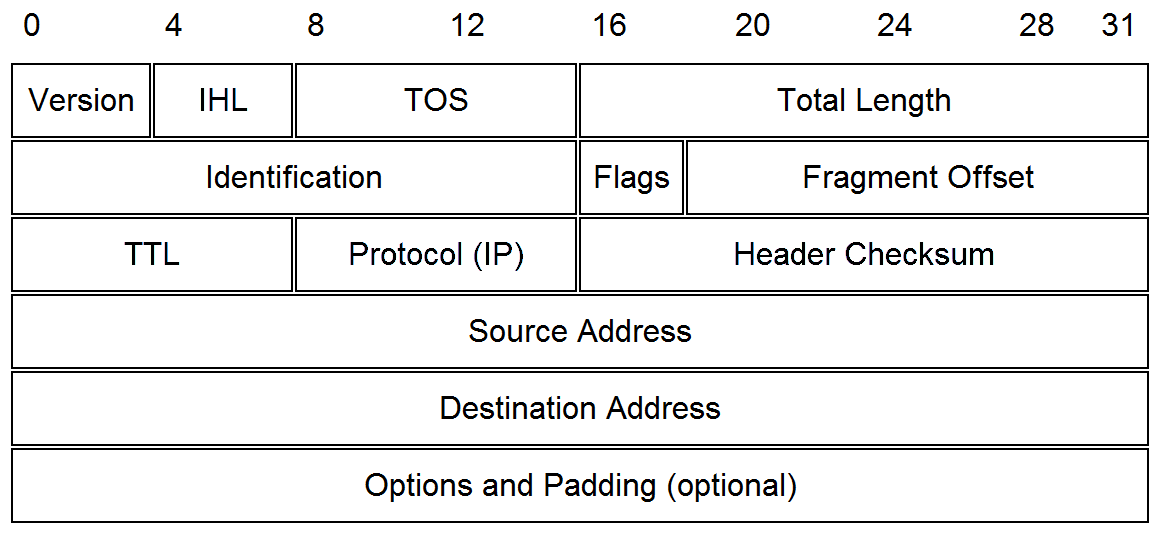
\includegraphics[width=0.7 \paperwidth]{./bilder/ippaket.png}
	\caption{IP Paket}
	\end{center}
	\end{minipage}
}
\end{center}
\end{figure}

Das erste Feld im Header ist eine Versionsnummer, dieses Feld ist 4 Bit lang und die einzig zurzeit gültigen Werte sind 4 für IPv4 und 6 für IPv6. Das nächste Feld heißt IP-Header-Length und gibt in Vielfachen von 32 Bit an, wie groß der Header ist. Das nachfolgende Feld Type-Of-Service kann für die Priorisierung von IP-Paketen genutzt werden. Das nächste Feld, Total-Length gibt die Gesamtgröße des IP-Paketes, inklusive Header, in Byte an. Da dieses Feld 16 Bit breit ist können IP-Pakete eine maximale Größe von 65.535 Bytes haben, werden die IP-Pakete jedoch per Ethernet übertragen so ist die Größe bereits durch die maximale Größe von Ethernet Paketen begrenzt (1500 Bytes). Die Felder Idendification, Flags und Fragment Offset werden benötigt um Daten, welche über mehrere IP-Pakete aufgeteilt (fragmentiert) wurden, wieder zusammensetzen zu können. Das nächste Feld TTL steht für Time-To-Live, es gibt quasi die noch restliche Lebenszeit des Paketes an. Dabei wird dieses Feld von jedem Router, den das Paket durchläuft, um 1 verringert, erreicht dieses Feld den Wert 0, so wird das Paket verworfen. Dieser Mechanismus soll sicherstellen, dass Pakete durch Fehler nicht im Kreis laufen und dadurch das Netzwerk auslasten und im schlimmsten Fall sogar überlasten. Das Protocol-Feld gibt das verwendete Protokoll auf der nächsthöheren Schicht an, dabei wird für UDP der Wert 17 und für TCP der Wert 6 verwendet. Die Header-Checksumme stellt wieder eine Prüfsumme für den Header, nicht aber für die Nutzdaten zur Verfügung. Diese Prüfsumme muss immer wieder neu berechnet und geschrieben werden, da sich die TTL mit jedem durchlaufen eines Knotenpunktes (Routers) ändert. Trotzdem nimmt das Berechnen dieser Prüfsumme recht viel Rechenzeit in Anspruch, weshalb moderne Router diese komplett ignorieren und den Wert nur um 1 erhöhen, aus diesen Gründen ist dieses Feld bei IPv6 nicht mehr vorhanden. Die Felder Source- und Destination-Address geben jeweils die Quell- und Ziel-IP-Adresse des IP-Paketes an, jede Adresse ist 32 Bit lang und liegt in der Network Byte Order vor. Zusätzlich können noch weitere Optionen und Flags folgen, diese müssen aber eine Größe von Vielfachen von 32 Bit aufweisen (eventuell mit einem Padding) und dürfen insgesamt höchstens 40 Bytes lang sein.

\newpage

\subsubsection{ARP}
Will man nun ein IP-Paket an eine bekannte IP-Adresse schicken, so ergibt sich folgendes Problem. Welche Ziel-MAC-Adresse soll im Ethernet Header angegeben werden, man weiß zwar die Ziel-IP-Adresse aber eben nicht die MAC-Adresse, diese wird aber benötigt. Hier kommt das sogenannte Address-Resolution-Protocol ins Spiel. Dieses sorgt dafür, dass das Netzwerkgerät die MAC-Adresse des Ziels herausfindet. Der Ablauf ist ungefähr folgender: ist die Ziel-MAC Adresse nicht bekannt, so wird ein ARP-Paket als Broadcast verschickt. In diesem steht quasi die Anfrage nach der MAC-Adresse zu einer passenden IP-Adresse. Fühlt sich nun ein Gerät im Netzwerk für diese IP-Adresse angesprochen, so antwortet es mit einem Paket, dieses mal nicht als Broadcast, im Paket steht nun als Quell-MAC-Adresse die vorher gesuchte MAC-Adresse zur angefragten IP-Adresse. Diese MAC-Adresse wird nun in einen Cache für eine gewisse Zeit geschrieben, damit man nicht bei jedem neuen IP-Paket diese ARP-Anforderung durchführen muss.

\newpage
\subsection{TCP}
Das Transmission-Control-Protocol bietet im Vergleich zu UDP Verbindungen, daher wird, bevor Daten übertragen werden können, ein Verfahren benötigt um die Verbindung aufzubauen, zudem muss die Verbindung am Ende wieder abgebaut werden. TCP enthält Mechanismen die sicherstellen, dass die Daten ankommen, dies wird durch erneutes Übertragen der Daten, beim Ausbleiben dieser, bewerkstelligt. Auch wird der Datenstrom bei TCP wieder in der richtigen Reihenfolge zusammengefügt. All diese Funktionen führen jedoch zu einem etwas größeren Header, sowie zu höherem Speicher- und Rechenaufwand im Netzwerkgerät.
\begin{figure}[h]
\begin{center}
\fbox{
	%Rahmengroesse	
	\begin{minipage}{0.6 \paperwidth}
	\begin{center}
	%Bildgroesse
	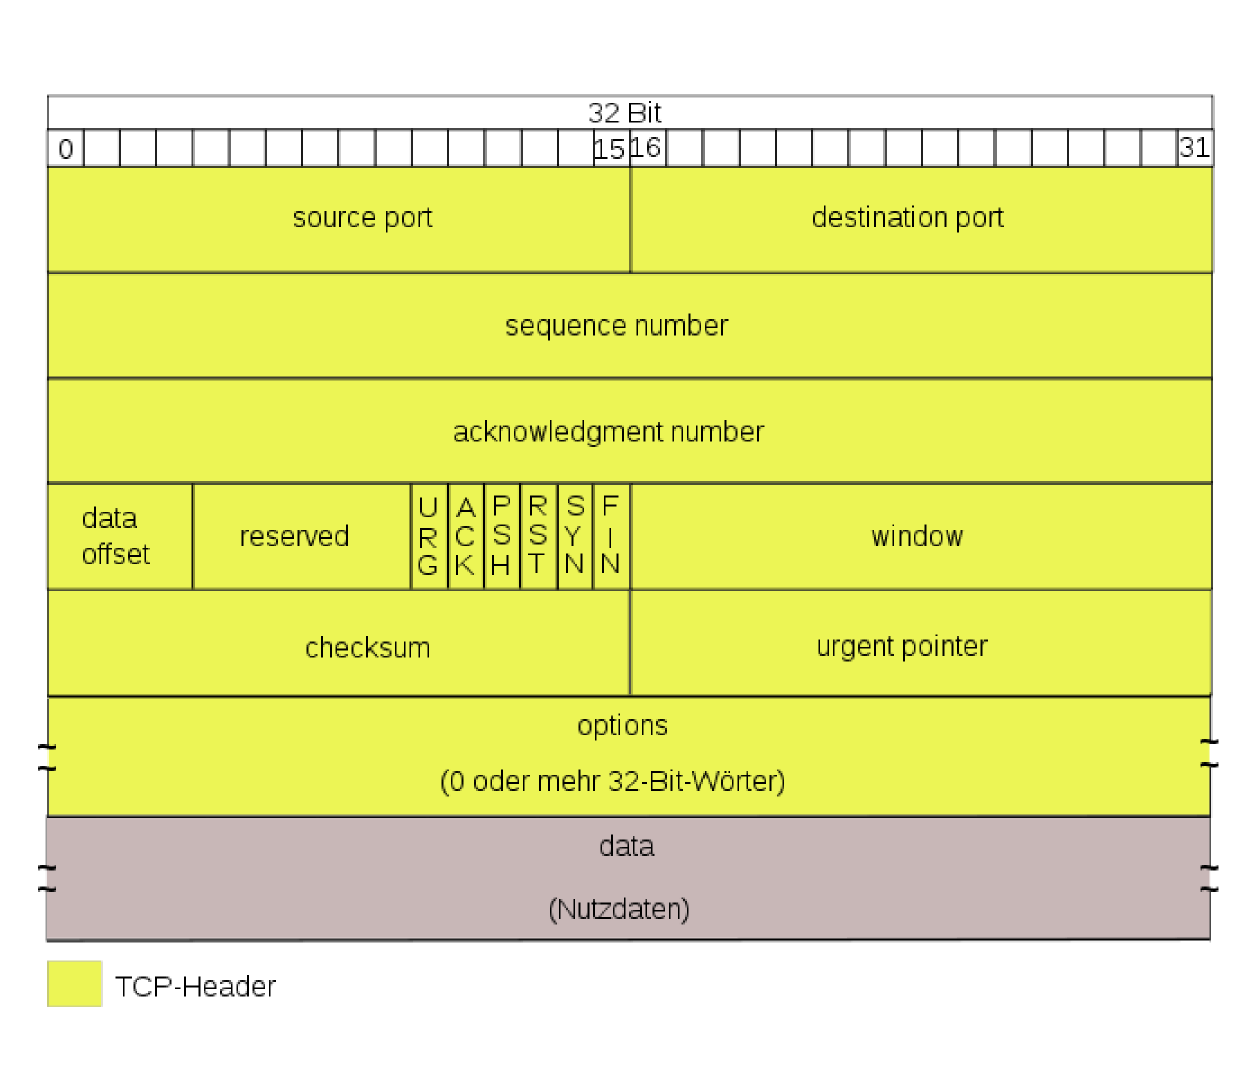
\includegraphics[width=0.6 \paperwidth]{./bilder/tcpheader.png}
	\caption{TCP Header}
	\label{tcp_header}
	\end{center}
	\end{minipage}
}
\end{center}
\end{figure}

Die Felder Source- und Destination-Port geben Auskunft darüber, von welchen Prozess bzw. an welchen Prozess dieses Paket gerichtet ist. Da die Pakete in unterschiedlicher Reihenfolge beim Empfänger ankommen können, müssen die Pakete im Empfänger wieder in der richtigen Reihenfolge zusammengesetzt werden. Dies wird durch die Sequence-Number erreicht, diese gibt Auskunft darüber, an welcher Stelle in dem Datenstrom sich das erste Byte der Nutzdaten befindet, somit ist im Empfänger eine Zusammensetzung der Pakete in der richtigen Reihenfolge möglich. Die Acknowledgement-Number gibt, falls das ACK-Flag gesetzt ist, an, welche Sequenznummer als letztes erfolgreich erhalten wurde, dies ist also quasi eine Bestätigung, dass der Datenstrom bis zu einer bestimmten Länge erfolgreich beim Empfänger angekommen ist. Das Feld Data Offset gibt die Länge des TCP Headers in Vielfachen von 32 Bit an, weiterhin existiert ein Reserved Feld, welches aber nicht verwendet wird, dieses Feld muss auf 0 gesetzt werden. Dann Folgt ein Feld mit den Control Flags, diese dienen zur Kennzeichnung bestimmter Zustände, welche für die Kontrolle und Aufrechterhaltung der Kommunikation benötigt werden.

\begin{itemize}
	\item URG: Ist das Urgent-Flag (urgent = wichtig), es soll besonders dringende TCP-Pakete kennzeichnen, findet aber heutzutage keine Verwendung mehr.
	\item ACK: Dieses Flag hat gemeinsam mit der Acknowledgement-Number die Aufgabe, bereits empfangene Pakete zu bestätigen.
	\item PSH: Dieses Flag dient dazu, den Puffer beim Empfänger zu umgehen, üblicherweise werden erst mehrere TCP-Pakete gepuffert und dann gemeinsam an die Anwendung übergeben. Ist dieses Flag jedoch gesetzt, so wird der Inhalt des Paketes, sofern die Reihenfolge stimmt, sofort an die Anwendung übergeben.
	\item RST: Das Reset-Flag wird verwendet, wenn eine Verbindung abgebrochen (nicht geschlossen) werden soll. Dies geschieht zum Beispiel bei technischen Problemen oder wenn unerwünschte Verbindungen nicht zu Stande kommen sollen.
	\item SYN: Dieses Flag dient der Synchronisation, es wird bei einem Verbindungsaufbau gesetzt, akzeptiert der Server die Verbindung antwortet er mit einem Paket in dem das SYN und das ACK Flag gesetzt ist. Will der Server die Verbindung verweigern, so antwortet er mit einem Paket in dem das RST-Flag gesetzt ist.
	\item FIN: Dieses Flag signalisiert, dass der Sender die Verbindung abbauen (Finish) und somit keine weiteren Daten mehr senden will.
\end{itemize}

Nach den Flags kommt das Feld (Receive)-Window, dieses Feld gibt in Byte an, wie viel der Sender bereit ist nach dem in Acknowledgement-Number erhaltenen Sequenzwert noch zu empfangen. Die Prüfsumme wird ähnlich wie bei UDP über die Nutzdaten, den TCP-Header und einen Teil des IP-Headers berechnet. Ist diese Prüfsumme falsch so wird das Paket verworfen, es wird zum Sender kein Paket mit einem ACK-Flag verschickt, somit wird das Paket erneut gesendet. Der Urgent-Pointer gibt an, bis zu welchem Byte im Paket sich die Daten befinden, die als urgent (wichtig) angesehen werden sollen, diese ermöglicht es in einem Paket mit dem Urgent-Flag auch die Übertragung von Daten, welche nicht als wichtig gekennzeichnet sind. Das letzte Feld kann wieder ähnlich wie bei UDP bis zu 40 Byte an Optionen enthalten.

\subsubsection*{Verbindungsaufbau und Verbindungsabbau}
Da TCP, wie bereits erwähnt, verbindungsorientiert ist, gibt es beim Verbinden und auch beim Abbauen der Verbindung eine bestimmte Vorgehensweise, der Aufbau und der Abbau einer Verbindung sind in dem folgenden Zustandsautomaten veranschaulicht:

\begin{figure}[h]
\begin{center}
\fbox{
	%Rahmengroesse	
	\begin{minipage}{0.7 \paperwidth}
	\begin{center}
	%Bildgroesse
	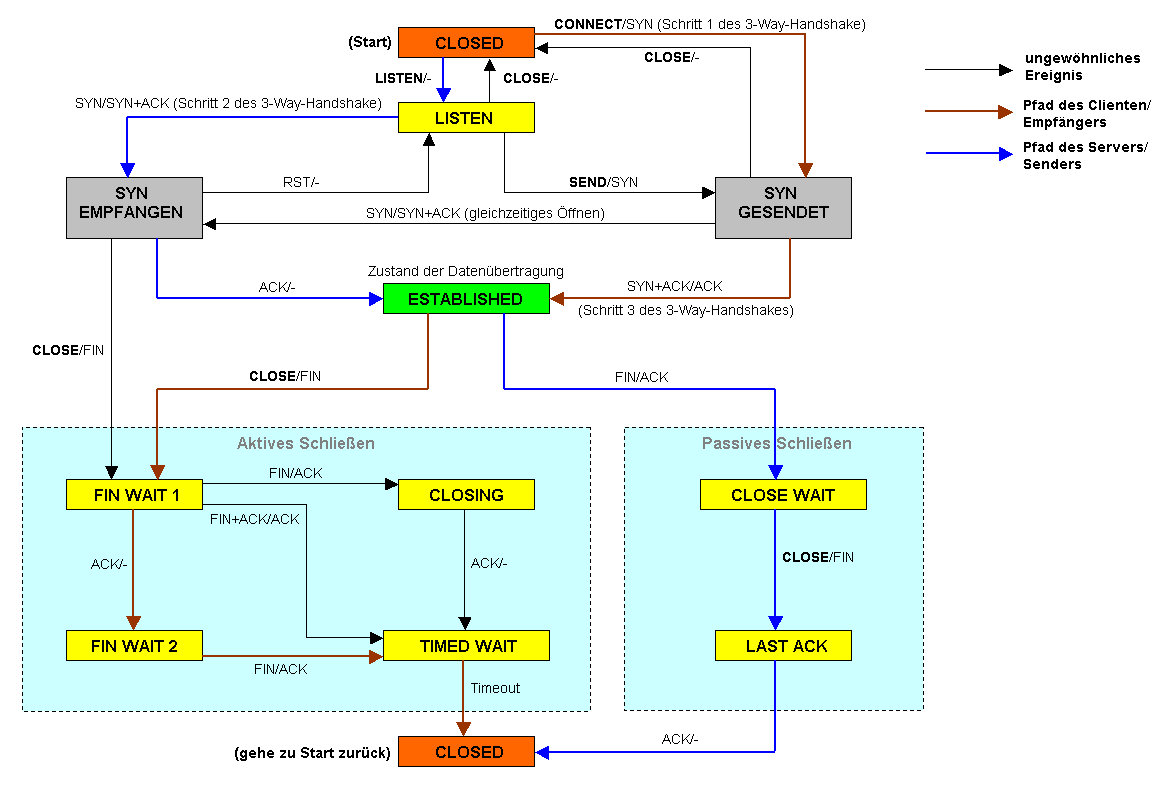
\includegraphics[width=0.65 \paperwidth]{./bilder/tcpconn.png}
	\caption{Auf- und Abbau einer TCP-Verbindung}
	\end{center}
	\end{minipage}
}
\end{center}
\end{figure}

Dabei ist der Ausgangszustand des Servers der Zustand LISTEN, in diesem Zustand wartet der Server auf ein TCP-Paket von einem Client. Dieses TCP-Paket muss das bereits erwähnte SYN-Flag gesetzt haben, ist dies der Fall, so antwortet der Server mit einem Paket, in welchem das SYN-Flag sowie auch das ACK-Flag gesetzt ist. Danach sendet der Client ebenfalls ein Paket in dem das SYN, sowie das ACK-Flag gesetzt sind, der Server antwortet darauf noch einmal mit einem ACK-Paket und die Verbindung ist erfolgreich aufgebaut, der Datenaustausch kann erfolgen.

Das Abbauen einer Verbindung wird üblicherweise vom Client eingeleitet, dieser führt das sogenannte aktive Schließen durch, indem er ein Paket mit dem FIN-Flag an den Server schickt, dieser leitet nun das passive Schließen ein und sendet erstmal an den Client ein ACK-Paket zurück. Der Client sendet noch ein FIN-Paket, woraufhin der Server dieses Paket abermals mit einem ACK bestätigt, jetzt ist die Verbindung geschlossen, die Ressourcen können nun freigegeben werden.

\newpage
\subsection{UDP}
Das User-Datagram-Protocol ist ein recht einfaches und auf IP basierendes Protokoll, es bietet keinen Verbindungsaufbau und keine Verbindungsabbau, zudem ist im Protokoll kein Mechanismus definiert, der die Ankunft von Daten oder die Richtigkeit der Reihenfolge sicherstellt. Will man dies erreichen, so muss man diese selber in Protokollen, welche auf UDP aufbauen, implementieren. Der Vorteil von UDP ist aber hingegen der kleinere Header, welcher zu einer höheren Effizienz der Bandbreite führt, weiterhin war UDP für diese Diplomarbeit vor allem von Bedeutung, da nur mit UDP die sogenannten Broadcasts möglich sind. UDP wird überall dort verwendet wo der Verlust von Paketen vernachlässigbar ist, dies ist zum Beispiel die Übertragung von Audio, Video und Sprache, ein UDP Paket ist folgendermaßen aufgebaut:
\begin{figure}[h]
\begin{center}
\fbox{
	%Rahmengroesse	
	\begin{minipage}{0.7 \paperwidth}
	\begin{center}
	%Bildgroesse
	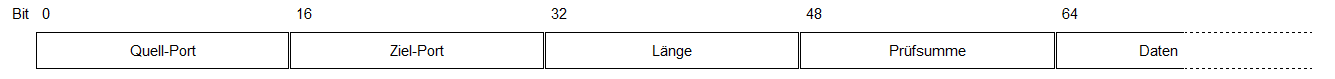
\includegraphics[width=0.7 \paperwidth]{./bilder/udpheader.png}
	\caption{UDP Paket}
	\end{center}
	\end{minipage}
}
\end{center}
\end{figure}

Auf dem Netzwerkgerät dient der Quell- und der Ziel-Port wieder zur Identifizierung des Prozesses von welchem das Paket kam, bzw. an welchen Prozess das Paket gerichtet war. Da UDP keine Verbindungen hat, kann der Quellport auf 0 gesetzt werden, falls keine Antwort empfangen werden muss. Die Länge gibt in Byte an, wie groß das UDP Paket ist, diese Länge bezieht den Header und die Nutzdaten mit ein. Die Prüfsumme ist optional, wenn sie nicht verwendet werden soll, wird ihr Wert auf 0 gesetzt, ansonsten wird die Prüfsumme über einen Teil des IP-Headers, den UDP-Header, und die Nutzdaten gebildet. In der Praxis wird diese Prüfsumme fast immer verwendet.


\subsection{DHCP}
DHCP steht für Dynamic-Host-Configuration-Protocol, durch dieses auf UDP basierende Protokoll wird es möglich, Netzwerkgeräte in ein bestehendes Netzwerk einzubinden, ohne dass diese vorher manuell konfiguriert werden müssen. Dabei sendet der Client beim Starten einen Broadcast, dieser wird von einem im Netzwerk befindlichen DHCP Server empfangen und verarbeitet. Über DHCP können unter anderem die IP-Adresse, die Netzwerkmaske, das Standardgateway, sowie der DNS-Server bezogen werden, neben diesen Optionen gibt es noch einige weitere, welche aber seltener verwendet werden, es kann zum Beispiel die Adresse eines Zeitservers angegeben werden. DHCP muss auf UDP aufbauen, da nur mit UDP die Broadcast-Pakete möglich sind, dabei wartet der Server auf Port 67 auf Anfragen, der Client erhält die Serverantworten auf Port 68 zurück. Zudem teilt der Server dem Client mit, wie lange ein sogenannter DHCP-Lease gültig ist, laut dem DHCP Protokoll muss nach der halben Zeit erneut eine Anfrage an den Server geschickt werden. Im Rahmen dieser Diplomarbeit wurde ein vollständiger DHCP Client implementiert, inklusive der Aktualisierung nach vorgegebener Zeit. Dazu musste aber die Framegröße des uIP Stacks auf 600 Byte erweitert werden.

\newpage
\section{Hardware [Pietryka]}
\subsection{Der Ethernet Controller}
\subsubsection{Auswahl des Ethernet Controllers}
Damit ein Mikrocontroller über das Ethernet kommunizieren kann, wird eine entsprechende Hardware benötigt, der sogenannte Ethernet Controller. Ein Ethernet Controller übernimmt dabei die Aufgaben der OSI-Schichten 1 (Physical) und 2 (Data-Link). Der Controller benötigt zudem einen entsprechend großen Empfangspuffer, um mindestens einen vollwertigen Ethernet-Frame (1542 Byte) aufzunehmen zu können. Dabei standen für 8-Bit Mikrocontroller vorerst zwei verschiedene Bausteine zur Auswahl, einmal der CP2200 von SiLabs, und einmal der ENC28J60 von Microchip. Beide Controller haben, was die Netzwerkkommunikation angeht, so ziemlich die selben Features, der gravierende Unterschied liegt jedoch in der Ansteuerung dieser. Der CP2200 wurde von SiLabs, wie es scheint, nur für die Verwendung mit einem Mikrocontroller vom Typ 8051 entwickelt, die Ansteuerung erfolgt deshalb über einen parallelen Adress-/Datenbus wodurch man mindestens 16 Leitungen und Pins am Mikrocontroller benötigt. Beim ENC28J60 erfolgt die Kommunikation über den SPI-Bus, daher benötigt man nur vier Leitungen (MOSI, MISO, SCK, CS), dadurch hat auch der Netzwerkcontroller selber nur 28 Pins und ist auch im "`bastlerfreundlichen"' DIP-Gehäuse zu bekommen. Dabei gilt die Parallele Übertragung als veraltet, diese wurde früher benutzt, weil die Prozessoren langsamer waren. Denn um die selbe Datenmenge in der selben Zeit mittels SPI zu übertragen braucht man einen 16 mal schnelleren Prozessor, dies ist heute kein Problem mehr. Ein anderer Faktor für die Auswahl des ENC28J60 war das Vorhandensein einer günstigen Entwicklungsplatine, es gibt bei Pollin den AVR-NET-IO Bausatz, dieser kostet nur \EUR{20} und enthält alle für die Netzwerkprogrammierung benötigten Komponenten(ATmega32, ENC28J60, RJ-45 Buchse).

\subsubsection{ENC28J60 Beschaltung}
Die Außenbeschaltung benötigt neben einigen Standardbauelementen auch einige 1\% Widerstände und einen 1:1 Übertrager, jedoch gib es RJ-45 Buchsen in denen bereits der Übertrager, sowie die LEDs bereits eingebaut sind.
\begin{figure}[h]
\begin{center}
\fbox{
	%Rahmengroesse	
	\begin{minipage}{0.7 \paperwidth}
	\begin{center}
	%Bildgroesse
	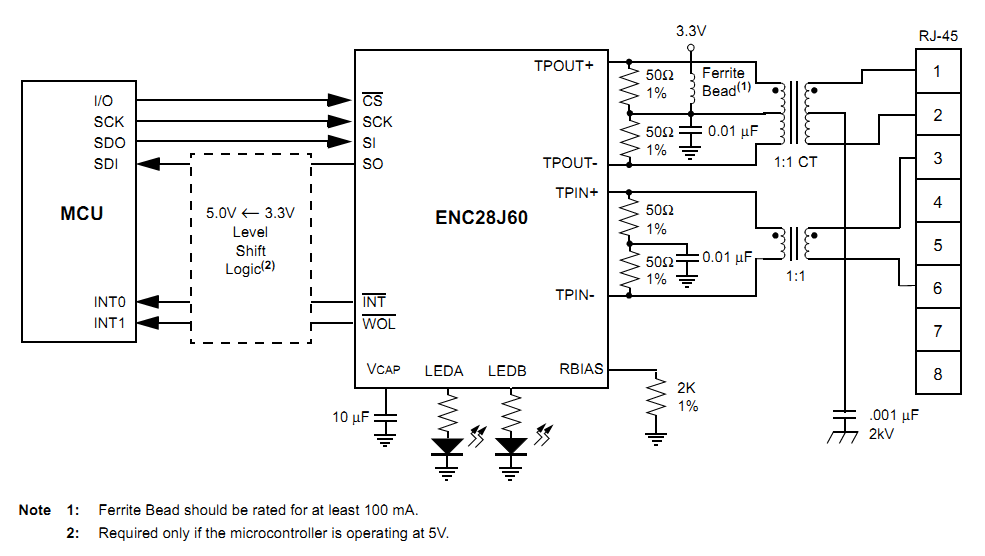
\includegraphics[width=0.7 \paperwidth]{./bilder/enc28j60_beschaltung.png}
	\caption{Aussenbeschaltung ENC28J60}
	\end{center}
	\end{minipage}
}
\end{center}
\end{figure}

\newpage

\subsubsection{ENC28J60 Treibersoftware}
Die erste Aufgabe war es, eine Bibliothek zu schreiben, welche es erlaubt, mithilfe des ENC28J60, Ethernet Pakete über das Netzwerk zu verschicken. Es waren zwar im Internet verschiedene Programme für den ENC28J60 vorhanden, diese waren aber teilweise schlampig und unschön geschrieben. Am Ende Stand eine von mir geschriebene Bibliothek zur Verfügung, die auch für andere Projekte genutzt werden kann, diese wurde für den AVR geschrieben und besteht aus zwei Dateien "`enc28j60.h"' und "`enc28j60.c"'. Zurzeit übernimmt die Bibliothek auch die Initialisierung des SPI-Busses. Will man dies verhindern, so muss man die Zeilen 187-197 in der Datei "`enc28j60.c"' entfernen, weiterhin wird es eventuell nötig sein, die  Pins für das Chip-Select anzupassen. Dazu muss man die Funktionen get\_cs() und release\_cs() in den Zeilen 24-32 ebenfalls anpassen. Für die Benutzung der Bibliothek stehen dann drei Funktionen zur Verfügung. Die Bibliothek selber findet sich im Ordner "`netcon Module/Pollin AVR-NET-IO/enc28j60/"' in den Dateien "`enc28j60.c"' und "`enc28j60.h"'.

Der Treiber selbst kann als stabil angesehen werden, es sind in den mehreren Monaten der Arbeit mit diesem keine Fehler aufgefallen, auch wurde die Geräte tagelang mit Erfolg getestet.

\newpage

\subsubsection*{void enc28j60\_init(const uint8\_t *mac\_addr)}
Initialisiert die Hardware des ENC28J60 mit der angegebenen MAC-Adresse, diese muss als ein Zeiger auf ein Array mit 6 Byte übergeben werden. Zurzeit wird auch die SPI-Hardware eines ATmega32 ebenfalls initialisiert, ist dies nicht gewünscht, so muss der Code entsprechend abgeändert werden.

\begin{quote}
\begin{verbatim}
const uint8_t mac_addr[6] = {0x02, 0x00, 0x00, 0x00, 0x00, 0x01};
enc28j60_init(mac_addr);
\end{verbatim}
\end{quote}

\subsubsection*{void enc28j60\_transmit(const uint8\_t *data, uint16\_t len)}
Sendet ein Ethernet-Paket in das Netzwerk, welches über einen Zeiger auf data referenziert wurde, mit der Länge len.
\begin{quote}
\begin{verbatim}
uint8_t buf[512];

strcpy(buf, "Das ist ein ungueltiges Paket");
enc28j60_transmit(buf, strlen(buf));
\end{verbatim}
\end{quote}

\newpage

\subsubsection*{uint16\_t enc28j60\_receive(uint8\_t *data, uint16\_t max\_len)}
Prüft, ob ein Paket im Puffer des ENC28J60 angekommen ist. Ist dies der Fall, so werden bis zu max\_len Bytes in den durch data referenzierten Bereich kopiert. Als Rückgabewert liefert die Funktion die Anzahl der erfolgreich gelesenen Bytes. Ist kein neues Paket beim Aufruf der Funktion vorhanden, so ist der Rückgabewert 0.
\begin{quote}
\begin{verbatim}
uint8_t buf[512], len;

while(1 > 0)
{
    len = enc28j60_receive(buf, 512);
    if(len > 1)
    {
        // Neues Paket
    }
}
\end{verbatim}
\end{quote}

\subsubsection{Ethernet-DK Port}
Weiterhin, wurde eine Portierung des ENC28J60 Treibers auf das Ethernet-DK von SiLabs durchgeführt. Dies lässt sich mit dem freien C-Compiler SDCC compilieren, die entsprechenden Projektdateien sind im Ordner "`netcon Module/Ethernet-DK/enc28j60"'. Damit dieses Projekt erfolgreich kompiliert, muss der SDCC Compiler entsprechen in der SiLabs IDE konfiguriert werden, zudem muss sowohl dem Linker als auch dem Compiler der Parameter "`--model-large"' übergeben werden.

\subsubsection{CP2200}
Auch wenn der CP2200 Ethernet-Controller nicht weiter verwendet wurde, so wurde ebenfalls ein Treiber geschrieben, sowie der uIP Stack auf diesen portiert, diese Projektdateien finden sich im Ordner "`netcon Module/Ethernet-DK/cp2200"'. Über die Stabilität kann keine Auskunft gegeben werden, jedoch hat die Netzwerkkommunikation über eine Stunde hinweg funktioniert. Auf eine weitere Dokumentation wird hier verzichtet, da der Treiber nur als Nebenprodukt verschiedener Experimente anzusehen ist.

\subsection{Pollin AVR-NET-IO}
Wie bereits erwähnt griffen wir für die Netzwerkentwicklung mit dem ENC28J60 auf einen Bausatz der Firma Pollin mit dem Namen AVR-NET-IO zurück. Dieser Bausatz bietet einen AVR ATmega32 Mikrocontroller, den ENC28J60 mit passender Ethernet-Buchse sowie der benötigte Außenbeschaltung. Die ursprüngliche Software, welche mit dem Bausatz ausgeliefert wurde, wurde nicht verwendet und überschrieben. Die Dokumentation dieses Bausatzes befindet sich auf der CD in der Datei "`AVR-NET-IO.pdf"'.

\newpage

\subsection{Zufallsgenerator}
Für das DHCP-Protokoll, sowie für das netfind-Protokoll wurde ein Zufallsgenerator benötigt, dabei bietet eine bereits beim AVR-Compiler mitgelieferte Bibliothek die Funktion eines Pseudozufallszahlengenerators. Dieser generiert eine immer gleiche Zahlenfolge, diese Zahlenfolge hängt vom einem Startwert(dem Seed) ab. Damit die Module nun unterschiedliche Zufallszahlen generieren, muss für den Generator ein wirklich zufälliger Seed gesetzt werden. Um eine wirklich zufällige Zahl für den Seed zu bekommen, wurde die Tatsache verwendet, dass der RAM-Speicher beim Einschalten mit zufälligen Werten befüllt ist. Dabei wird der Speicher vom absoltuten Ende bis zum Ende des Bereiches wo globale Variablen bereits initialisiert wurden durchlaufen, die einzelnen Speicherplätze werden miteinander XOR-Verknüpft. Diese Funktion sieht folgendermaßen aus:
\begin{quote}
\begin{verbatim}
uint16_t get_seed(void)
{
    uint16_t seed = 0;
    uint16_t *p = (uint16_t *) (RAMEND + 1);
    extern uint16_t __heap_start;

    while(p >= &__heap_start + 1)
        seed ^= *(--p);
    return seed;
}
\end{verbatim}
\end{quote}

Der zurückgelieferte Wert wird dem Zufallszahl-Generator der AVR-Bibliothek übergeben, somit hat man die Möglichkeit auf unterschiedlichen Modulen und nach dem Neustarten unterschiedliche Zufallszahlenfolgen zu erhalten.


\subsection{Der uIP TCP/IP Stack}
Die Kommunikation der Module soll im Netzwerk über TCP ablaufen, zum einen damit gewährleistet ist, dass die Daten auch ankommen, zum anderen damit die Module mit allen Betriebssystemen, Programmiersprachen und Netzwerkbibliotheken kompatibel sind, denn dies ist nur durch TCP oder UDP der Fall, diese Protokolle sind in jedem modernen Betriebssystem ein fester Bestandteil. Eine Software die sich nun um das IP, TCP und eventuell auch um das UDP Protokoll kümmert, nennt man einen TCP/IP Stack.

Der von uns verwendetet Ethernet-Controller liefert uns jedoch nur Ethernet-Frames, daher benötigt man einen in Software geschriebenen TCP/IP Stack. Einen solchen zu schreiben wäre an sich schon eine eigene Diplomarbeit, hinzu kommt noch die Tatsache, dass RAM-Speicher und Rechengeschwindigkeit des Mikrocontrollers begrenzt sind, das Ganze soll auf einem ATmega32 mit 2K RAM laufen.

Ein hierfür entwickelter TCP/IP Stack ist der uIP Stack von Adam Dunkels. Dieser wurde genau für die oben genannten Anforderungen entwickelt und ist komplett in C geschrieben, und zwar plattformunabhängig. Der Austausch der Ethernet-Frames zwischen dem ENC28J60 Treiber und dem Stack erfolgt über einen globalen Puffer, welcher in unserem Fall eine Größe von 600 Byte hat. Zudem ist es möglich, die Routinen, welche zur Berechnung der Prüfsummen benutzt werden, selber, zum Beispiel in Assembler, zu implementieren, um hier eventuell Geschwindigkeitsvorteile rauszuholen. Der Stack beherrscht die Kommunikation über UDP und TCP und erlaubt mehrere eingehende sowie ausgehende Verbindungen. Durch die Eigenheit des Stacks müssen Programme die den Stack benutzen als sogenannte Zustandsautomaten programmiert werden. Wenn ein Paket an einem für eine Anwendung bestimmten Port angekommen ist, so wird eine vorher definierte und vom Benutzer geschriebene Callback-Funktion aufgerufen. Diese Funktion verarbeitet nun das Paket und sendet eventuell eine Antwort. Es muss aber nicht unbedingt ein hereingekommenes Paket der Auslöser für einen Aufruf dieser Funktion sein, diese Funktion wird auch zum Beispiel alle 100ms automatisch aufgerufen um es dem Benutzer zu ermöglichen eventuelle Verwaltungsaufgaben zu erledigen.

Im Grunde sieht der Aufbau der Callback-Funktion folgendermaßen aus:
\begin{quote}
\begin{verbatim}
void generic_app_call(void)
{
    if(uip_newdata()) {
        // Neue Daten
    }
    
    if(uip_rexmit()) {
        // Beim Übertragen der TCP-Daten ist ein
        // Fehler aufgetreten, die Daten müssen
        // neu gesendet werden
    }
    
    if(uip_poll()) {
        // Ereignis wird alle 100ms aufgerufen
    }
}
\end{verbatim}
\end{quote}

\newpage

Neben den hier im Beispiel aufgeführten Ereignissen uip\_newdata(), uip\_rexmit() und uip\_poll() gibt es noch weitere Ereignisse, auf diese wird aber jetzt nicht näher eingegangen, die weiteren Ereignisse sind in der uIP Dokumentation ganz gut beschrieben, welche sich in dem "`uip-1.0.tar.gz"' Archiv findet.

Um selber Daten mit Hilfe des uIP-Stacks zu schicken gibt es die Funktion "`void uip\_send(const void * data, int len)"', diese Funktion sendet die Daten über die aktuelle Verbindung, dabei wird ein Zeiger auf die Daten, sowie deren Länge übergeben. Diese Funktion lässt sich nur innerhalb einer der oben erwähnten Callback-Funktionen nutzen. Will man kontinuierlich Daten senden, geht dies nur höchstens alle 100ms, wenn die Callback-Funktion aufgerufen wird.

\newpage

\subsection{DHCP Implementierung}
Da aufgrund des uIP Stacks die DHCP-Implementierung als ein Zustandsautomat erfolgen musste, wurden folgende Zustände definiert:

DHCP\_BOOT\_WAIT: In diesem Zustand verbleibt das Gerät nach dem Einschalten eine zufällige Zeit lang (2-5 Sekunden).

DHCP\_DISCOVER: Es wird ein Discover-Paket gesendet, dieses wird als Broadcast verschickt und dient dazu einen oder mehrere DHCP-Server im Netzwerk zu finden.

DHCP\_OFFER: Es wird auf eine Angebot (Offer) von einem oder mehreren DHCP-Servern gewartet, dabei wird immer das erste Angebot gewählt. Das Offer-Paket vom DHCP-Server enthält bereits alle benötigten Daten wie IP-Adresse, Subnetzmaske, etc.

DHCP\_REQUEST: Das Netzwerkmodul sendet nun eine Anfrage an den Server ob es die IP-Adresse für sich beanspruchen kann.

DHCP\_ACK: Es wird nun auf eine Zustimmung (Acknowledge) des DHCP-Servers gewartet, kommt dieses an, so werden die Parameter wie IP-Adresse, Subnetzmaske, etc. auf das Netzwerkgerät übernommen und für die weitere IP-Kommunikation verwendet.

DHCP\_WAIT\_RENEW: Die DHCP-Implementierung verweilt in diesem Zustand bis die halbe Lease-Time abgelaufen ist, denn dann muss eine sogenannte Erneuerung (Renew) stattfinden, diese Erneuerung der Daten läuft aber genauso ab wie beim ersten Mal.

\newpage
In einem Diagramm dargestellt sieht dieser Zustandsautomat folgendermaßen aus:
\begin{figure}[h]
\begin{center}
\fbox{
	%Rahmengroesse	
	\begin{minipage}{0.6 \paperwidth}
	\begin{center}
	%Bildgroesse
	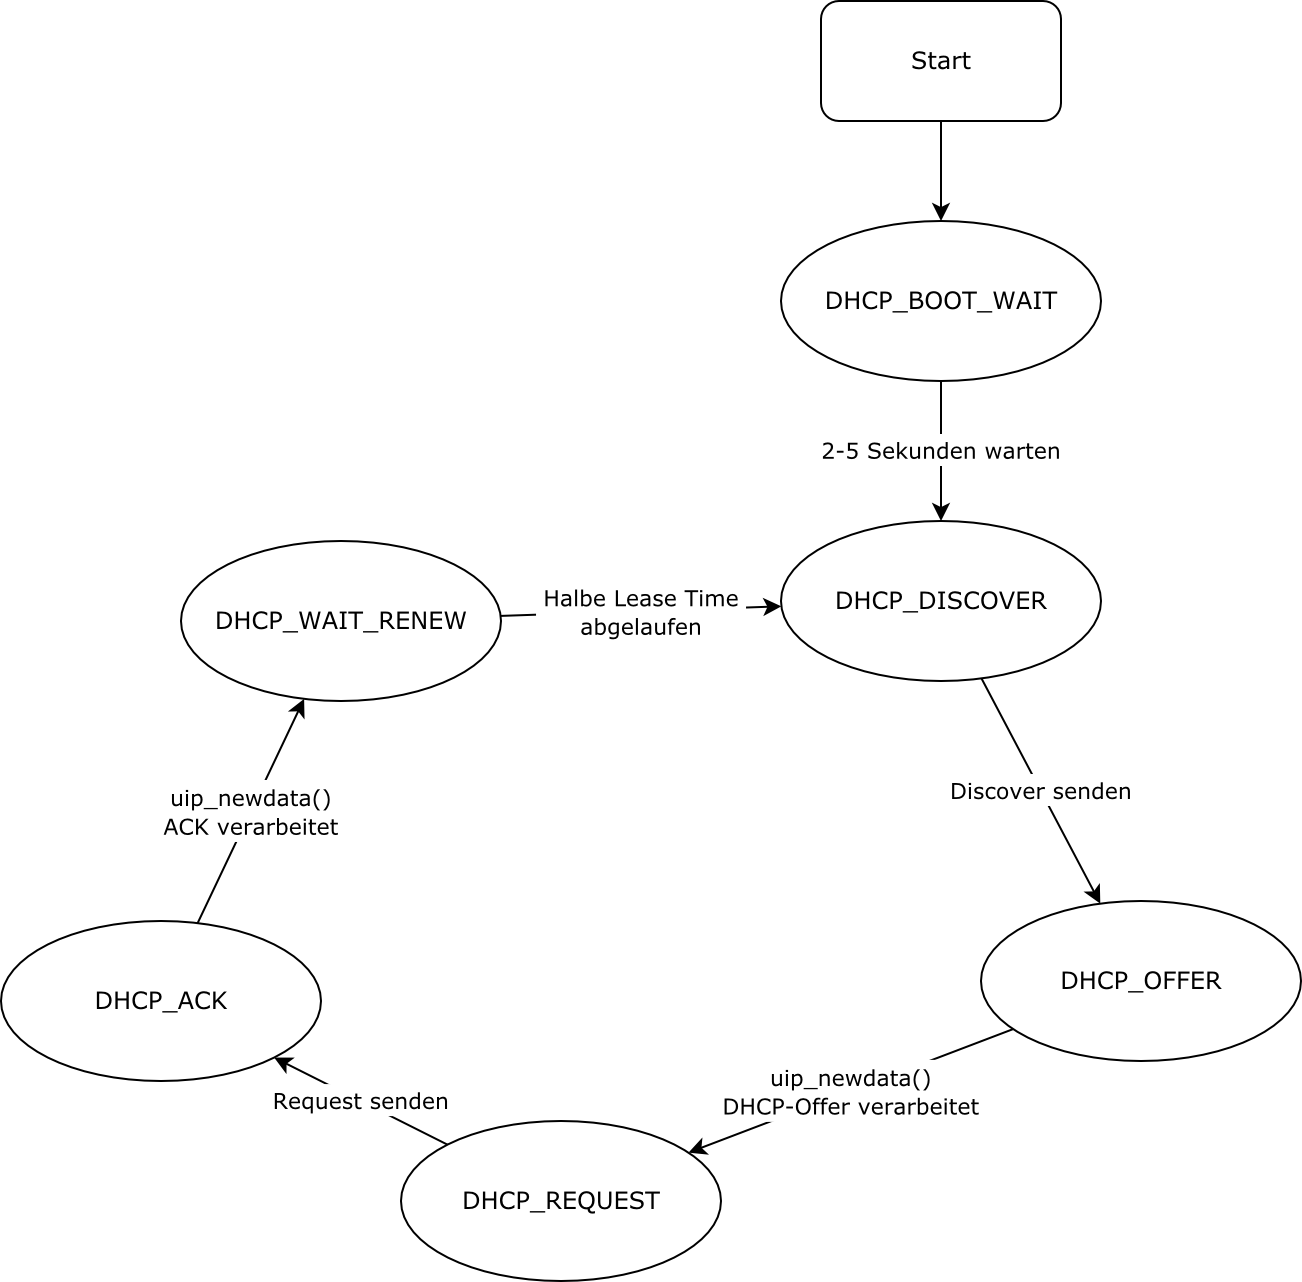
\includegraphics[width=0.6 \paperwidth]{./bilder/dhcp_state_machine.png}
	\caption{DHCP-Client Zustandsautomat}
	\end{center}
	\end{minipage}
}
\end{center}
\end{figure}


Da bei DHCP Broadcasts verwendet werden, basiert dieses Protokoll auf dem UDP-Protokoll, dabei lauscht der Server auf dem Port 67 auf Anfragen, der Client erhält die Antworten der DHCP-Server am Port 68. Auf den konkreten Code wird hier nicht weiter näher eingegangen, eine vollständige DHCP-Implementierung findet sich im Ordner "`netcon Module/Pollin AVR-NET-IO/netcon"' in den Dateien "`dhcp.c"' und "`dhcp.h"'.

\subsection{netcon Serial Protocol}
Wie bereits erwähnt, war es eines der Ziele, ein Netzwerkmodul zu entwickeln, welches es erlaubt andere Messgeräte "`einfach"' in das Messsystem einzubinden. Dazu kommuniziert das Netzwerkmodul mit dem Messgerät über die serielle Schnittstelle nach einem bestimmten Protokoll, dem netcon Serial Protocol. Die Messgeräte verhalten sich dabei passiv und erhalten vom Netzwerkmodul verschiedene Anfragen, diese sollten innerhalb von 50ms entsprechend beantwortet werden. Jegliche Kommunikation läuft dabei über den standardmäßigen ASCII-Zeichensatz und mit einer Symbolrate von 9600 Baud ab.

\begin{figure}[h]
\begin{center}
\fbox{
	%Rahmengroesse	
	\begin{minipage}{0.7 \paperwidth}
	\begin{center}
	%Bildgroesse
	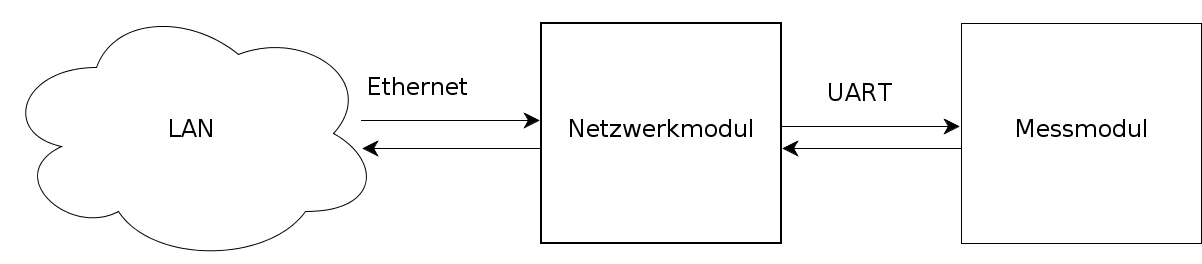
\includegraphics[width=0.7 \paperwidth]{./bilder/aufbau13.png}
	\caption{UART Schnittstelle}
	\end{center}
	\end{minipage}
}
\end{center}
\end{figure}


Kommandos:
\begin{quote}
\begin{verbatim}
Anfrage: n
Antwort: <Name>\n
Fragt den Namen des Messgerätes ab.

Anfrage: o
Antwort: <Standort>\n
Fragt den Standort des Messgerätes ab.

Anfrage: a
Antwort: <Anzahl>\n
Fragt die Anzahl der Sensoren, die mit dem Messgerät gemessen
werden können ab, wobei Anzahl eine Zahl von 00-FF sein kann.

Anfrage: w##
Antwort: <Wert>\n
Fragt den aktuellsten Messwert von dem Sensor mit der Nummer
## ab (## im Bereich von 00-FF).

Anfrage: f##
Antwort: <Format>\n
Fragt das Format für den Wert von Sensor ## ab.
Dieses gibt als ASCII-Zeichen an, wie der Wert
an das Netzwerkmodul übergeben wird, folgende
Formate sind vorgesehen:
    h - Hexadezimal
    i - Dezimal
    f - Fließkommazahl
    
Anfrage: t##
Antwort: <Typ>\n
Fragt den Typ für den Sensor ## ab, dies soll es ermöglichen,
bei der Ausgabe nach Temperatursensoren, Luftdrucksensoren,
etc. zu filtern. Der Typ ist eine Zahl von 00-FF, jedoch
wurden noch keine Typen definiert, außer 00 für Spannung
definiert.

Anfrage: m##
Antwort: <Minimum>\n
Fragt das Minimum des Sensors ## ab.

Anfrage: x##
Antwort: <Maximum>\n
Fragt das Maximum des Sensors ## ab.
\end{verbatim}
\end{quote}

Beim Einschalten des Netzwerkmoduls werden zuerst der Name, der Ort und die Anzahl der Sensoren abgefragt, anschließend wird für jeden Sensor das Format, der Typ, der Min- und der Max-Wert abgefragt. Nach dieser Initialisierung werden alle 500ms die aktuellen Werte aller Sensoren nacheinander abgefragt. Eine Implementierung dieses Protokolls befindet sich im Ordner "`netcon Module/Pollin AVR-NET-IO/netcon\_ser"' in den Dateien "`serconn.c"' und "`serconn.h"', diese Implementierung wurde noch nicht einem dauerhaften Test unterzogen, es könnten noch Fehler enthalten sein.

\newpage

\subsection{nefind Protocol}
Da man die Module in ein bestehendes Netzwerk mit möglichst wenig bis gar keinem Konfigurationsaufwand einbinden soll, musste ein Protokoll entwickelt werden, welches es dem netcond-Daemon erlaubt, angeschlossene Module im Netzwerk zu finden. Dieses Protokoll basiert auf Broadcasts und baut deshalb auf UDP auf. Um die Module im Netzwerk zu finden, muss der Daemon eine Broadcaspaket mit dem Zielport 50000 senden, diese Anfrage muss folgendermaßen aussehen:
\begin{figure}[h]
\begin{center}
\fbox{
	%Rahmengroesse	
	\begin{minipage}{0.7 \paperwidth}
	\begin{center}
	%Bildgroesse
	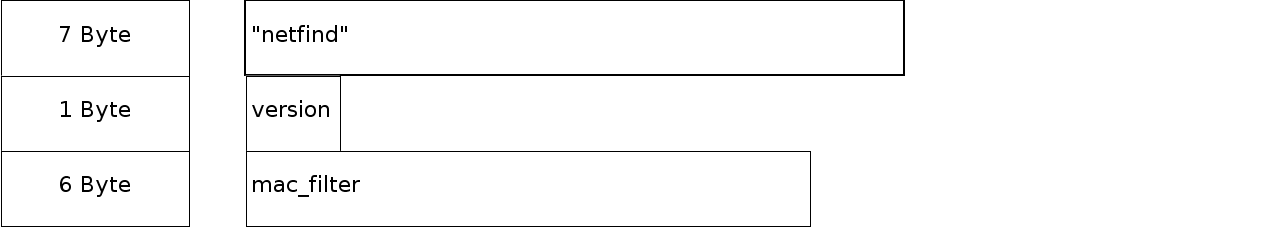
\includegraphics[width=0.7 \paperwidth]{./bilder/netfind_anfrage.png}
	\caption{netfind-Anfrage}
	\label{netfind_anfrage}
	\end{center}
	\end{minipage}
}
\end{center}
\end{figure}

"`netfind"' ist eine ASCII-Zeichenkette mit dem selben Inhalt, diese Zeichenkette dient zur Erkennung des Paketes, das Feld "`version"' ist für eventuelle Unterscheidungen bei zukünftigen Protokollversionen vorgesehen, die einzige zurzeit gültige Version ist 0. Zuletzt erlaubt es das Feld "`mac\_filter"', nach Netzwerkmodulen mit bestimmten MAC-Adressen im Netzwerk zu suchen, dabei vergleicht das Netzwerkmodul seine eigene MAC-Adresse mit der im Paket angegebenen Adresse, ist diese nicht gleich, so sendet dieses Modul keine Antwort. Sollen alle Module gefunden werden, der Filter also nicht aktiv sein, so muss dieses Feld auf den Wert FF:FF:FF:FF:FF:FF gesetzt werden.

\newpage

Nach dieser Anfrage antworten die verschiedenen Netzwerkmodule innerhalb von 1-3 Sekunden, dabei wird der exakte Zeitpunkt zufällig gewählt um die Broadcasts im Netzwerk etwas über die Zeit zu verteilen, die Antwort eines Moduls hat den folgenden Aufbau:
\begin{figure}[h]
\begin{center}
\fbox{
	%Rahmengroesse	
	\begin{minipage}{0.7 \paperwidth}
	\begin{center}
	%Bildgroesse
	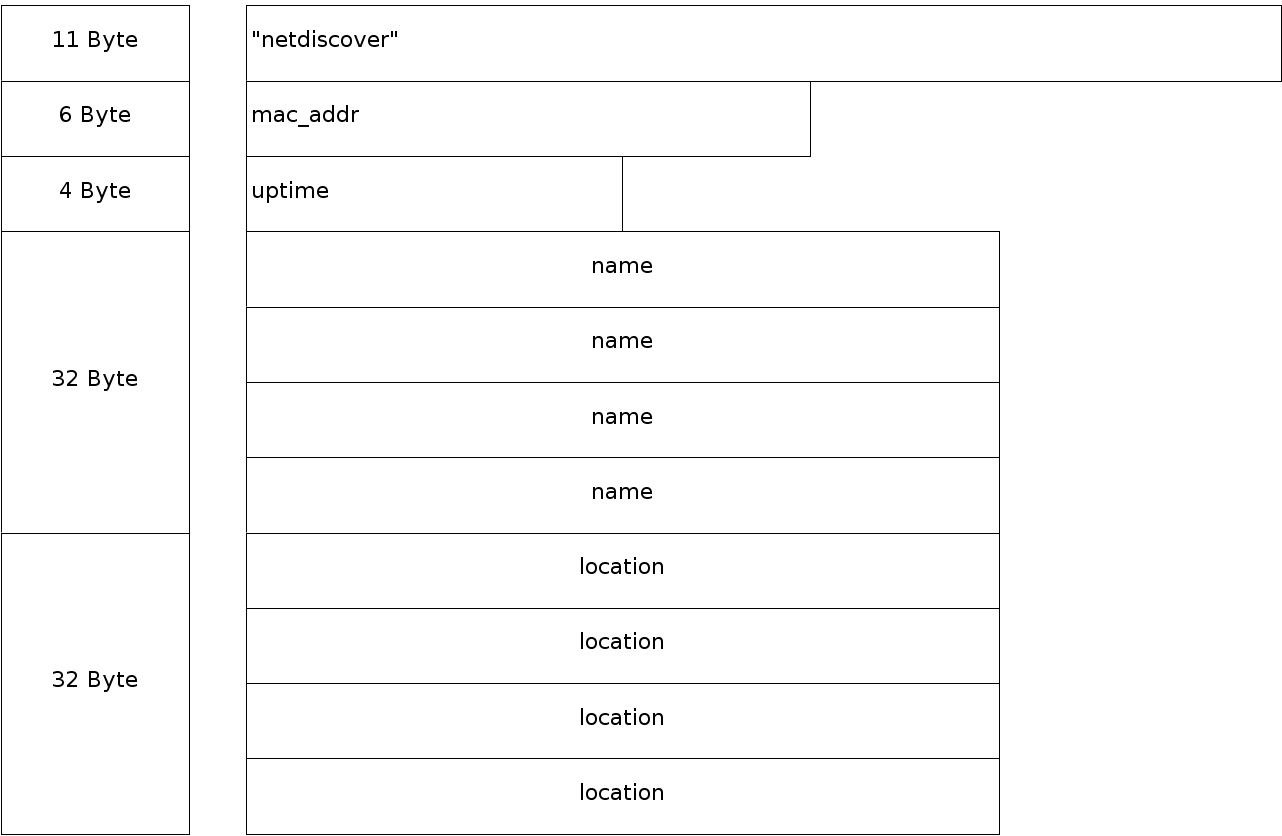
\includegraphics[width=0.7 \paperwidth]{./bilder/netfind_antwort.png}
	\caption{netfind-Antwort}
	\label{netfind_antwort}
	\end{center}
	\end{minipage}
}
\end{center}
\end{figure}

\newpage

"`netfind"' ist ebenfalls wieder eine ASCII-Zeichenkette, welche signalisiert, dass es sich bei dem Paket um ein netfind-Antwortpaket handelt. Das Feld "`mac\_addr"' enthält die 6-Byte lange MAC-Adresse des entsprechenden Moduls. Als nächstes Feld folgt die '`uptime"', dieses Feld enthält die Zeit, welche seit dem Start des Moduls vergangen ist. Diese Zeit ist in 10ms Schritten angegeben und ist ein Ganzzahlwert in der Network-Byte-Order. Die beiden letzten Felder '`name"' und '`location"' geben jeweils den Namen und den Standort des Modules an, dabei handelt es sich um bis zu 32-Byte lange ASCII-Zeichenketten, welche aber vorzeitig mit einer Nullterminierung (Bytewert 0) abgeschlossen werden können. Somit können beide Felder effektiv nur mit 31 Byte belegt werden, das letzte Byte muss die Nullterminierung sein.

Eine Implementierung dieses Protokolls findet sich in dem Ordner "`netcon Module/Pollin AVR-NET-IO/netcon"' in den Dateien "`netfind.c"' und "`netfind.h"', diese Implementierung ist vollständig getestet und funktionsfähig.

\newpage

\subsection{netcon Protocol}
Das letzte für diese Diplomarbeit entwickelte Protokoll dient dazu, es dem netcond-Daemon zu ermöglichen, die Messwerte der Module einzuholen. Damit diese Messwerte auch sicher ankommen, basiert dieses Protokoll auf TCP. Dabei lauscht das Netzwerkmodul am TCP Port 50003 auf eingehende Verbindungen, kommt nun eine TCP-Verbindung zustande, so kann der netcond-Daemon über das GET-Kommando verschiedene Daten des Moduls abfragen. Ein GET-Kommando sieht folgendermaßen aus:

\begin{quote}
\begin{verbatim}
GET <key>\r\n
\end{verbatim}
\end{quote}

Dabei handelt es sich um eine ASCII-Zeichenkette, wobei \textbackslash r und \textbackslash n, das Carriage-Return sowie das Line-Feed ASCII-Zeichen repräsentieren.

Das Modul antwortet nun im Erfolgsfall mit:
\begin{quote}
\begin{verbatim}
OK\r\n
<value>\r\n
\end{verbatim}
\end{quote}
und im Fehlerfall mit:
\begin{quote}
\begin{verbatim}
ERROR\r\n
\end{verbatim}
\end{quote}

Für den \textless key\textgreater Wert gibt es nun eine Liste von verschiedenen Parametern, welche abgefragt werden können.

\begin{quote}
\begin{verbatim}
NAME        Fragt den Namen des Moduls ab.

PLACE       Fragt den Standort des Moduls ab.

UPTIME      Fragt die Laufzeit des Moduls in 10ms ab,
            dieses Mal als ASCII-Zeichenkette.
            
DEVICECOUNT Fragt die Anzahl der Sensoren ab, welche
            für das Gerät vorhanden sind. Die
            Nummerierung dieser erfolgt jedoch von 0.

TYPE ##     Fragt den Typ für den Sensor ## ab, dies 
            soll es ermöglichen, bei der Ausgabe nach
            Temperatursensoren, Luftdrucksensoren, etc.
            zu filtern. Der Typ ist eine Zahl von
            00-FF, jedoch wurden noch keine Typen, außer
            00 für einen Spannungswert, definiert.
            
DTYPE ##    Fragt das Format für den Wert von Sensor ## ab.
            Dieses gibt an, in welchem Format die Werte
            geliefert werden. Mögliche Formate sind dafür:
                h - Hexadezimal
                i - Dezimal
                f - Fließkommazahl
                
MIN ##      Fragt den Minimalwert für den Sensor ## ab,
            dies wird benötigt um eine Balkendarstellung
            zu ermöglichen.
            
MAX ##      Fragt den Maximalwert für den Sensor ## ab.

MAX         Liefert die 6-Byte lange MAC-Adresse des Moduls
            im Format XX:XX:XX:XX:XX:XX.
            
VALUE ##    Liefert den letzten Messwert des Sensors ## in
            dem entsprechenden Format.
\end{verbatim}
\end{quote}
Eine beispielhafte Kommunikation könnte folgendermaßen aussehen, wobei D der netcond-Daemon ist und M das Modul:
\begin{quote}
\begin{verbatim}
D: GET NAME\r\n
M: OK\r\n
   Testmodul\r\n
   
D: GET DEVICECOUNT\r\n
M: OK\r\n
   4\r\n
   
D: GET TYPE 0\r\n
M: OK\r\n
   00\r\n
   
D: GET DTYPE 0\r\n
M: OK\r\n
   f\r\n
   
D: GET VALUE 0\r\n
M: OK\r\n
   4.75\r\n
\end{verbatim}
\end{quote}

\newpage

Da sich im Betrieb außer den Messwerten diese Parameter nicht ändern werden, empfiehlt es sich, um die Belastung zu reduzieren, die Parameter für Name, Standort, Datentyp, etc. nur am Anfang bei der Initialisierung abzufragen. Lediglich den VALUE-Parameter muss man zwangsweise immer wieder für alle Sensoren abrufen. Eine vollständige Implementierung dieses Protokolls findet sich im Ordner "`netcon Module/Pollin AVR-NET-IO/netcon"' in den Dateien "`netcon.c"' und "`netcon.h"', diese wurde während der Entwicklung ausführlich getestet und kann als stabil angesehen werden. Für die Zukunft ist eventuell noch ein SET Kommando vorgesehen um zum Beispiel ein Licht ein- oder auszuschalten.

\newpage

\subsection{Kompilieren der Quelldateien}
Eine bereits kompilierte Version der Quelldateien findet sich in den Unterordnern von "`netcon Module/Pollin AVR-NET-IO"' im Unterordner "`bin"', diese Hexfiles können dann beispielsweise mit avrdude auf den AVR mit dem folgenden Befehl auf der Kommandozeile gebrannt werden:
\begin{quote}
\begin{verbatim}
avrdude.exe -p atmega32 -P com3 -c stk500v2 -U flash:w:main.hex
\end{verbatim}
\end{quote}

Der COM-Port sowie eventuell der Programmer-Typ (hier STK500v2) müssen entsprechend angepasst werden.

Will man Veränderungen an den Quelltexten vornehmen, so muss man diese neu kompilieren, hierbei kommen sogenannte Makefiles zum Einsatz, dafür sind jedoch einige Vorbereitungen nötig, welche im Folgenden erläutert werden.

\subsubsection{Installation der AVR-Toolchain}
Die AVR-Toolchain kommt vom Atmel und liefert einen vollständigen C-Compiler, sowie die grundlegenden Bibliotheken zur AVR-Programmierung. Die Installationsdatei "`avr-toolchain-installer-3.3.0.710-win32.win32.x86.exe"' befindet sich auf der CD, mit dieser Version der Toolchain wurden die Quelltexte erfolgreich kompiliert, andere Versionen der Toolchain könnten funktionieren, wurden aber nicht getestet. Es empfiehlt sich, die Toolchain in das Standardverzeichnis "`C:/Program Files/Atmel/AVR Tools/AVR Toolchain/"' zu installieren.

\subsubsection{Avrdude installieren}
Avrdude ist ein Konsolenprogramm, welches es ermöglicht, die erzeugten Hexfiles mithilfe eines Programmers auf den Mikrocontroller zu programmieren. Damit dieser Schritt später komfortabler abläuft, sollten die Dateien "`avrdude.exe"' und "`avrdude.conf"' aus dem "`avrdude.zip"' Archiv in den bin-Ordner der Toolchain Installation kopiert werden. Hat man bei der Installation den Standardpfad behalten, so sollte die "`avrdude.exe"' folgenden Pfad besitzen: "`C:/Program Files/Atmel/AVR Tools/AVR Toolchain/bin/avrdude.exe"'

\subsubsection{Installation von Cygwin}
Da der Buildvorgang hier auf sogenannten Makefiles basiert, wird ein Makefile-Interpreter, das Programm make, benötigt, dieses wird mit Cygwin mitgeliefert. Cygwin selber bietet eine Linuxähnliche Arbeitsumgebung auf einem Terminal unter Windows. Die Cygwin Installationsdatei findet sich entweder auf der CD unter dem Namen "`cygwin-setup.exe"', oder kann direkt von der Cygwin-Webseite http://www.cygwin.com/ heruntergeladen werden. Die Installation ist selbsterklärend, jedoch sollte man bei der Paketauswahl das Paket "`make"' mitinstallieren, dies enthält das benötigte Programm. Nach der Installation kann man ein Cygwin-Terminal starten, es sollte jedoch hierbei auf die Pfade geachtet werden. Will man zu einem Windows-Pfad navigieren, so muss man den Laufwerksbuchstaben nicht als "`X:"' angeben sondern als "`/cygdrive/X/"', weiterhin werden Ordner in den Pfaden wie bei Linux üblich durch ein "`/"' getrennt.

Als Beispiel sei hier folgender Windows Pfad gegeben:
\begin{quote}
\begin{verbatim}
C:\Program Files\Atmel\AVR Tools\AVR Toolchain\bin
\end{verbatim}
\end{quote}
dieser Pfad würde in Cygwin der folgenden Schreibweise entsprechen:
\begin{quote}
\begin{verbatim}
/cygdrive/C/Program Files/Atmel/AVR Tools/AVR Toolchain/bin
\end{verbatim}
\end{quote}
daher der Befehl um im Cygwin-Terminal in diesen Ordner zu wechselnd würde folgendermaßen lauten:
\begin{quote}
\begin{verbatim}
cd /cygdrive/C/Program Files/Atmel/AVR Tools/AVR Toolchain/bin
\end{verbatim}
\end{quote}

\subsubsection{Kompilieren}
Hat man bei der Installation der AVR-Toolchain einen anderen Pfad angegeben, so muss man diesen jetzt im entsprechenden Makefile des Projektes anpassen, der Pfad muss in der Zeile 41 entsprechend geändert werden, dabei muss dieser in der Cygwin-Schreibweise angegeben werden. Weiterhin kann man in der Zeile 277 und 280 den Programmer und den COM-Port für avdude anpassen. Sind diese Anpassungen vorgenommen worden, so kann man nun mit dem Cygwin-Terminal in den Projektordner navigieren und mit:
\begin{quote}
\begin{verbatim}
make
\end{verbatim}
\end{quote}
den Kompiliervorgang starten. Dabei entsteht eine "`main.hex"' Datei, welche nun zum Beispiel mit avrdude durch folgenden Aufruf in den Mikrocontroller programmiert werden kann:
\begin{quote}
\begin{verbatim}
make program
\end{verbatim}
\end{quote}
Am Schluss kann man noch die temporären und überflüssigen Dateien mit einem Aufruf von:
\begin{quote}
\begin{verbatim}
make clean
\end{verbatim}
\end{quote}
löschen, dadurch werden alle Dateien (inklusive Hexfile) gelöscht, welche beim Kompilieren erzeugt worden sind.

\subsection{Inbetriebnahme}
Nachdem das Programm in den AVR gebrannt worden ist, kann nun das Pollin-AVR-NET-IO Kit in Betrieb genommen werden. Hat man das Projekt "`netcon Module/Pollin AVR-NET-IO/netcon"' kompiliert und in den AVR programmiert, so muss man nur mehr das Netzwerkkabel an das Netzwerk anschließen und das Kit mit einer 9V Versorgung in Betrieb nehmen. Das Kit fordert nun die IP-Adresse per DHCP an und ist dann bereit, Kommandos vom netcond-Daemon zu erhalten. Es stehen dann die Werte der internen ADCs der Kanäle 0 und 1 zur  Verfügung.

Hat man hingegen das Projekt "`netcon Module/Pollin AVR-NET-IO/netcon\_ser"' auf den AVR programmiert, so muss man an die Pins RXD (Pin 14) und TXD (Pin 15) des ATmega32 ein entsprechendes RS232 Gerät anhängen, welches sich an das netcon Serial Protocol hält.

\newpage
\section{Software [Lipp]}

Das Kapitel beschreibt das Softwareinterface zwischen den Modulen und den Applikationen zur Anzeige der Moduldaten, um eigene Anwendungen, wie Webseiten oder Smartphone-Apps zu realisieren. Als Anwendungsbeispiel wurde bereits eine Website implementiert, die für den eigenen Gebrauch herangezogen werden kann.

\subsection{Aufgaben}
Die Software, genauer gesagt \textbf{netcond}, ist ein sogenannter Daemon (Hintergrundprozess), der im Allgemeinen die Module im Netzwerk verwaltet, indem er ihre Messwerte aufzeichnet, die über ein spezielles Interface abgefragt werden können. Auch modulseitig kommt ein eigens entwickeltes Protokoll zum Einsatz, das bereits im vorangegangenen Kapitel erklärt wurde. Wenn sich alle Module nach dieser Spezifikation verhalten, werden sie auch von netcond als solche erkannt.

\subsection{Java}

Die Anwendung wurde in Java geschrieben, um Plattformunabhängigkeit zu gewährleisten. Damit ist der Einsatz auf jeder Plattform möglich, die eine Java Runtime Environment (JRE) in Version 6 oder höher zur Verfügung stellt, egal ob PC, Server oder Embedded System. Die Installation dieser Laufzeitumgebung ist im Kapitel \textbf{Installation} genau beschrieben. 

\newpage

\subsection{Hardwareanforderungen}
Netcond wurde für hardwareschwache Computer konzipiert. Demnach steht dem Einsatz auf eingebetteten Systemen nichts im Wege, Voraussetzung ist ausschließlich, wie bereits erwähnt, die Verfügbarkeit der JRE. 

Da der Daemon im Hintergrund läuft, muss das Betriebssystem über keine grafische Oberfläche verfügen. Netcond kann auf einem Server/Embedded System ohne Monitor über zum Beispiel SSH ausgeführt und gewartet werden. 

\textbf{Empfohlende Hardware}

\begin{itemize}
	\item 1 GHz CPU
	\item 128 MB RAM (nur für netcond)
	\item Netzwerkkarte
	\item Textbasiertes Betriebssystem mit SSH-Zugang
\end{itemize}

Soll eine eigene Website oder die dieser Diplomarbeit für die Anzeige der Moduldaten genutzt werden, ist weiters ein PHP-fähiger Webserver, wie zum Beispiel Apache erforderlich. Wenn dieser auf der selben Hardware laufen soll, wird zusätzlich Arbeitsspeicher benötigt. Die Installation eines Webservers wird im Abschnitt \textit{Installation} für die gängigen Betriebssysteme beschrieben. 

\newpage

\subsection{Funktionsweise}

Grunsätzlich ist die Funktionsweise des Java-Daemons netcond in einem Absatz beschrieben:

Nach dem Start sucht der Main-Thread alle paar Sekunden das Netzwerk nach verbunden Modulen ab und hält diese in einer Liste. Für jedes dieser Module wird ein neuer Programmfaden erzeugt, der ständig Messdaten abfragt und diese speichert. Zusätzlich startet der Daemon einen weiteren Subprozess, die Schnittstelle, über die eine Anwendung - in diesem Fall z.B. ein Webserver - die Daten abfragen kann. Verbindet sich ein Webbrowser zu diesem Webserver, weist ein PHP-Script den Daemon an, die aktuellen Daten zu übermitteln. Diese werden dann auf der Website angezeigt. Dieses Prinzip ist noch einmal in Abb. \ref{funktionsweise} grafisch verdeutlicht.

\begin{figure}[h]
\begin{center}
\fbox{
	%Rahmengroesse	
	\begin{minipage}{0.7 \paperwidth}
	\begin{center}
	%Bildgroesse
	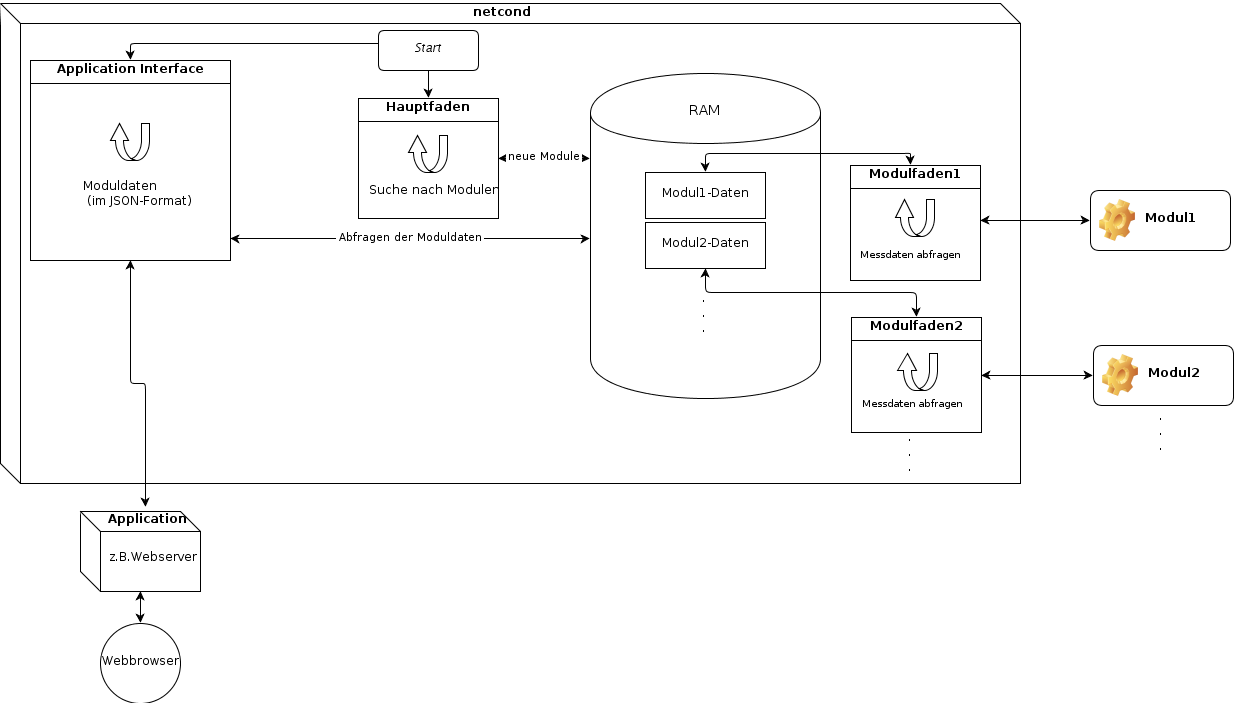
\includegraphics[width=0.7 \paperwidth]{./bilder/funktionsweise.png}
	\caption{netcon - Funktionsprinzip}
	\label{funktionsweise}
	\end{center}
	\end{minipage}
}
\end{center}
\end{figure}
\newpage

\subsection{Aufbau}

Nun folgt die Beschreibung des Quellcodes wobei Kentnisse in Java erforderlich sind.\footnote{Der Quellcode von netcond ist im Verzeichnis netcon Software/netcond zu finden. Weiters kann der gesamte Ordner als Projekt in Eclipse importiert werden, um am Quellcode Anpassungen vorzunehmen.} Erläutert werden dabei nicht die Programmzeilen im einzelnen, sondern für das Verständnis relevante Programmteile. Die Verwendung der netcon API Schnittstelle für die Programmierung eigener Anwendungen ist im nächsten Kapitel beschrieben: 

Der Sourcecode besteht aus einigen Java-Klassen bzw. -Dateien, die in Paketen organisiert sind. Auf oberster Ebene, sind das \textbf{lib}, die Programmbibliothek und \textbf{program}, die Programmthreads. Diese sind je nach Funktion wiederum in mehrere Unterpakete unterteilt (siehe Abb. \ref{software_aufbau}).

\begin{figure}[h]
\begin{center}
\fbox{
	%Rahmengroesse	
	\begin{minipage}{0.5 \paperwidth}
	\begin{center}
	%Bildgroesse
	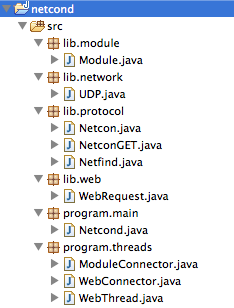
\includegraphics[width=0.3 \paperwidth]{./bilder/software_aufbau.png}
	\caption{netcond - Übersicht Sourcecode}
	\label{software_aufbau}
	\end{center}
	\end{minipage}
}
\end{center}
\end{figure}

\newpage

\subsubsection*{lib.network}

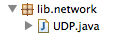
\includegraphics[width=0.17 \paperwidth]{./bilder/lib_network.png}

Dieses Paket enthält die statische Klasse UDP.java, die rudimentäre UDP-Funktionen zum Senden und Empfangen von Daten- und Broadcastpaketen bereitstellt. 

Die Funktion sendPacket() dient dazu ein einfaches UDP-Paket zu verschicken. Dazu nimmt sie die zu sendende Nachricht \textit{msg}, die Zieladresse \textit{dstAdr} (vom Typ InetAddress), Zielport \textit{dstPort} und den Quellport \textit{srcPort} als Parameter. Die Angabe des Quellports ist erforderlich, damit der Empfänger auf anwendungsspezifische Pakete filtern kann.

\begin{quote}
\begin{verbatim}

public static void sendPacket
(String msg, InetAddress dstAdr, int dstPort, int srcPort) 

\end{verbatim}
\end{quote}

Die Funktion receivePacket() empfängt ein UDP-Paket. Dazu benötigt sie als Parameter den Zielport des zu empfangenden Pakets \textit{lstPort} und den Timeout - also die Zeit bis der Empfangversuch abgebrochen wird - in Millisekunden und liefert das empfangene Paket in Form eines DatagramPacket zurück.

\begin{quote}
\begin{verbatim}

public static DatagramPacket 
receivePacket(int lstPort, int timeout)

\end{verbatim}
\end{quote}

\newpage

Für das Versenden von Broadcast-Paketen wird die überladene Funktion sendBroadcast() verwendet, die als Parameter entweder einen String, oder ein Byte-Array bekommt, sowie den Ziel- und Quellport des Pakets.

\begin{quote}
\begin{verbatim}

public static void 
sendBroadcast(String msg, int dstPort, int srcPort)

public static void 
sendBroadcast(byte msg[], int dstPort, int srcPort)

\end{verbatim}
\end{quote}

Die letzte Funktion der UDP-Klasse receiveBroadcast() empfängt Broadcast-Pakete, wobei sie den Zielport des Broadcast-Pakets als Parameter bekommt und das empfangene Paket als DatagramPacket zurückliefert.

\begin{quote}
\begin{verbatim}

public static DatagramPacket receiveBroadcast(int lstPort)

\end{verbatim}
\end{quote}

\newpage

\subsubsection*{lib.module}

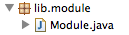
\includegraphics[width=0.17 \paperwidth]{./bilder/lib_module.png}

Das Paket lib.module enthält die Klasse Module.java, dessen Instanzen reale Module im Netzwerk abbilden. Diese bestehen aus folgenden Attributen:

\begin{quote}
\begin{verbatim}

private String hostname;
private String location;
private String ip;
private int port;
private String mac;

private String uptime;

private int devicecount;		
private int type[];				
private String value[];			
private String minValue[];	
private String maxValue[];		
private String dtype[];			
	
private ModuleConnector thread;	

\end{verbatim}
\end{quote}

\newpage

Ein Modul besitzt demnach einen Hostnamen, wie z.B. \textit{Temperaturmodul}, einen Standort, IP, Port und MAC. Die Uptime zeigt an, wie lange das Modul bereits online ist. Wie bereits im vorherigen Kapitel erwähnt kann ein Modul aus mehreren sogenannten Devices bzw. Sensoren bestehen, deren Anzahl in der Instanzvariablen \textit{devicecount} gepspeichert wird. Je nachdem wie groß diese Zahl ist (max. 9) enthält das \textit{type}-Array die Messtypen und das \textit{value}-Array die aktuellen Messwerte der einzelnen Devices. Die zwei weiteren Felder \textit{minValue[]} und \textit{maxValue[]} enthalten die minimalen und maximalen Messwerte der Devices während \textit{dtype[]} anzeigt in welchem Datentyp die Messgrößen vorliegen. 

Die letzte Variable \textit{thread} ist an dieser Stelle wahrscheinlich noch nicht ganz verständlich, sei vollständigkeitshalber aber trotzdem erwähnt: Um die Messwerte der Devices abzufragen wird nach Erstellung der Instanz - also nach Auffinden eines Moduls - ein Thread gestartet, der über TCP mit dem Modul kommuniziert. Dazu benötigt jedes Modulobjekt seine eigene Threadvariable vom Typ ModuleConnector. Näheres dazu im Abschnitt \textit{program.threads}. 

Zusätzlich zu den Getter- und Setter-Methoden für jede Variable besteht die Klasse Module noch aus folgenden Methoden:

\begin{quote}
\begin{verbatim}

public void startThread() 

\end{verbatim}
\end{quote}

Diese Methode legt ein Objekt vom Typ ModuleConnector an und startet damit den Modulthread um die Messwerte abzufragen. Sozusagen eine Setter-Methode für die Instanzvariable thread.  

\newpage

\begin{quote}
\begin{verbatim}

public JSONObject getJSON()

\end{verbatim}
\end{quote}

Die Methode getJSON() liefert die Moduldaten, also die Werte der Instanzvariablen verpackt in einem JSONObject zurück. 

JSON ist ein ein kompaktes, einfach lesbares Datenformat, das speziell für den Datenaustausch zwischen Anwendungen erfunden wurde. Der Aufbau eines JSON-Objekts ist im Kapitel netcon API genau beschrieben, da es die Grundlage für die Schnittstelle zwischen netcond und anderen Anwendungen bildet. Hier sei noch erwähnt, dass Java in der Grundausstattung keine JSON-Klassen mitbringt und diese Funktionalität mit Bibliotheken von Drittanbietern nachgerüstet werden muss. In diesem Fall wurde JSON.simple, ein einfaches Toolkit für JSON eingebunden, um JSON-text zu encodieren und decodieren.

Jede (nichtstatische) Klasse besitzt einen Konstruktor, auch die Module-Klasse. Der Konstruktor wird bekanntlich beim Erstellen eines Objektes aufgerufen. Dies geschieht beim Auffinden eines Moduls im Hauptthread. Dazu mehr im Abschnitt \textit{program.main}. Beim Aufruf werden die Werte aller Parameter an die erstellten Instanzvariablen übergeben, während devicespezifische Daten (devicecount, type[], value[], minValue[], maxValue[], dtype[]) und die uptime zunächst auf Standardwerte initialisiert (0, null) und erst später durch den Modulthread laufend gesetzt werden. 
\begin{quote}
\begin{verbatim}

public Module
(String hostname, String location, InetAddress ip, 
int port, String mac)

\end{verbatim}
\end{quote}

\subsubsection*{lib.protocol}

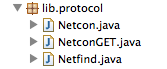
\includegraphics[width=0.2 \paperwidth]{./bilder/lib_protocol.png}

Im Kapitel Hardware wurden bereits die definierten Protokolle für das Auffinden und Abfragen von Modulen im Netzwerk beschrieben. Dazu enthält das Paket lib.protocol die statischen Klassen Netfind.java und Netcon.java. 

Die Klasse Netfind enthält zwei Funktionen, netfind() und netdiscover(). Netfind() erzeugt ein Byte-Array, das die entsprechend dem Protokoll definierten Daten eines Netfind-Pakets zum Auffinden der Module enthält. Im Protokoll vorgesehen, aber nicht weiter genutzt, ist auch ein MAC-Filter, der im Programm auf den Standardwert FF:FF:FF:FF:FF:FF gesetzt wurde. 

Der zweiten Funktion netdiscover() kann ein DataPacket übergeben werden, das zuallererst auf Richtigkeit des Protokolls geprüft wird. Danach werden die Moduldaten entpackt und eine neues Modul - also eine Instanz der Klasse Modul - erzeugt und zurückgeliefert.

\begin{quote}
\begin{verbatim}

public static byte[] netfind() 
public static Module netdiscover(DatagramPacket packet)

\end{verbatim}
\end{quote}

\newpage
Das netcon-Protokoll dient zur Kommunikation zwischen netcond und den Modulen, vorallem um sich veränderliche Daten, wie Messwerte aufzuzeichnen. Dazu besitzt die Klasse Netcon die Funktion netcon(), die den gewünschten Befehl vom enum-Typ NetconGET und die Devicenummer als Parameter erhält und ein Byte-Array mit den Daten zur Anfrage an ein Modul zurückliefert. 

\begin{quote}
\begin{verbatim}

public static byte[] netcon(NetconGET c, String device)

\end{verbatim}
\end{quote}

Die Auswahlmöglichkeiten für den enum-Parameter sind in der enum-Klasse NetconGET definiert. Einfacher gesagt lassen sich all diese Daten von einem Modul über das Netcon-Protokoll abrufen.  


\begin{quote}
\begin{verbatim}

public enum NetconGET {

	    uptime, name, devicecount, devicetype, 
	    value, min, max, dtype;

}

\end{verbatim}
\end{quote}

\newpage

\subsubsection*{lib.web}

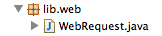
\includegraphics[width=0.2 \paperwidth]{./bilder/lib_web.png}

Im Paket lib.web enthalten ist die statische Klasse WebRequest.java, mit der Funktion get(). Diese dient zur Verarbeitung der Anfragen von anderen Anwendungen. 

\begin{quote}
\begin{verbatim}

public static JSONObject get(String request)

\end{verbatim}
\end{quote} 

Als Parameter bekommt die Funktion get() den zweiten Wert der GET-Anfrage einer Drittanwendung (z.B. einer Website) \textit{request} als String und liefert ein JSONObject zurück, das die Daten für die weitere Verarbeitung oder Anzeige enthält. Bisher versteht die Funktion nur den Befehl zur Abfrage aller Moduldaten und Messwerte. Dazu legt die Funktion ein JSON-Array an, geht die Modulliste durch, ruft für jedes Modul die bereits beschriebene Instanzmethode getJSON() auf und fügt die Daten dem JSON-Array nacheinander hinzu. Ist die Modulliste leer gibt sie ein spezielles JSON-Object zurück. Bei einer undefinierten GET-Anfrage liefert die Funktion \textit{null} zurück. 

\newpage

\subsubsection*{program.threads}

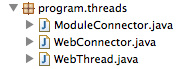
\includegraphics[width=0.22 \paperwidth]{./bilder/lib_threads.png}

Das Paket program.threads enthält drei Klassen, die jeweils einen anderen Thread definieren. 

Ein Thread der Klasse ModuleConnector wird wie bereits beschrieben, für jedes hinzugefügte Modul gestartet, um mit dem realen Modul zu kommunizieren und Messwerte abzufragen. Den Ablauf zeigt Abb. \ref{moduleconnector}.

\begin{figure}[h]
\begin{center}
\fbox{
	%Rahmengroesse	
	\begin{minipage}{0.8 \paperwidth}
	\begin{center}
	%Bildgroesse
	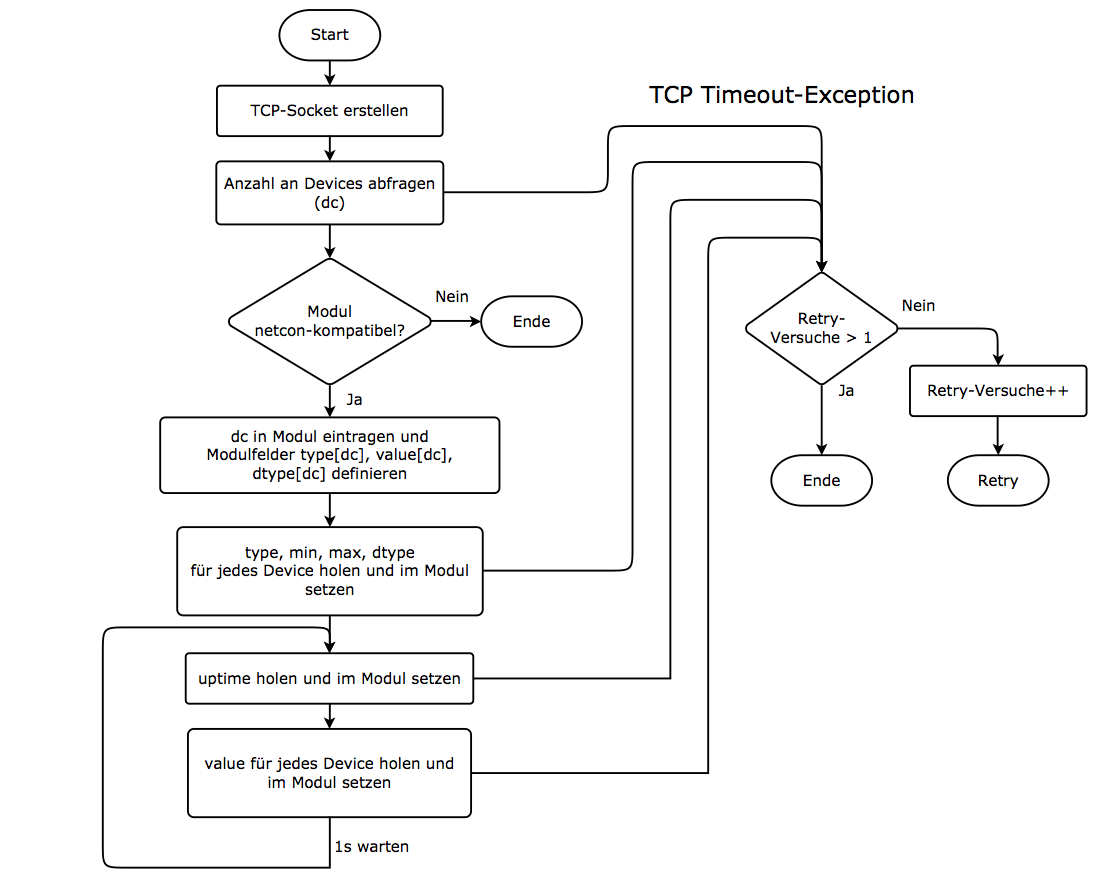
\includegraphics[width=0.61 \paperwidth]{./bilder/moduleconnector.png}
	\caption{ModuleConnector-Thread}
	\label{moduleconnector}
	\end{center}
	\end{minipage}
}
\end{center}
\end{figure}

\newpage

Nachdem also ein Modul im Netzwerk gefunden und ein Objekt erstellt wurde, wird sein ModuleConnector-Thread gestartet. Dieser erstellt einen TCP-Socket (Port 50003) mit den javainternen Bibliotheken und versucht anschließend per TCP die Anzahl der Devices abzufragen. Erhält er vom realen Modul keine netcon-konforme Antwort, wird er beendet. Im anderen Fall definiert er die Instanzvariable \textit{devicecount} und erstellt die Felder der Instanz, da jetzt die Anzahl der Devices bekannt ist. In der nächsten TCP-Anfrage holt der Thread \textit{type}, \textit{min}, \textit{max} und \textit{dtype} für jedes Device und weist sie den Instanzvariablen zu. Danach beginnt eine Endlosschleife, in der die \textit{uptime} und \textit{value} (Messwert) geholt und gesetzt werden, wobei ein Delay von einer Sekunde eingebaut wurde. Alle TCP-Anfragen werfen bei längerer Wartezeit eine Timeout-Exception. Eine Variable für die Retry-Versuche wird dann um 1 inkrementiert und ein weiterer Versuch gestartet, vorausgesetzt die Variable war nicht größer als 1. Die Retry-Versuche sind je TCP-Anfrage gültig, deshalb wird die Variable auch vor jeder Anfrage neu definiert. Wird der ModulThread im Programmblauf an einer Stelle beendet, wird der offene TCP-Socket geschlossen und das Modulobjekt gelöscht.

Der WebConnector-Thread bildet die Schnittstelle zu Drittanwendungen, wobei er für jede Anfrage einen Thread der Klasse WebThread startet und die Daten des Requests übergibt, um gleich darauf auf die nächste Anfrage zu warten. Die WebThreads bearbeiten die Anfragen mithilfe der Funktionen aus dem lib.web Paket, leiten die Antwort im JSON-Format an die Drittanwendung weiter und werden daraufhin beendet. Das Ablaufdiagramm in Abb. \ref{webconnector} macht diesen Vorgang verständlicher. 

\newpage

\begin{figure}[h]
\begin{center}
\fbox{
	%Rahmengroesse	
	\begin{minipage}{0.8 \paperwidth}
	\begin{center}
	%Bildgroesse
	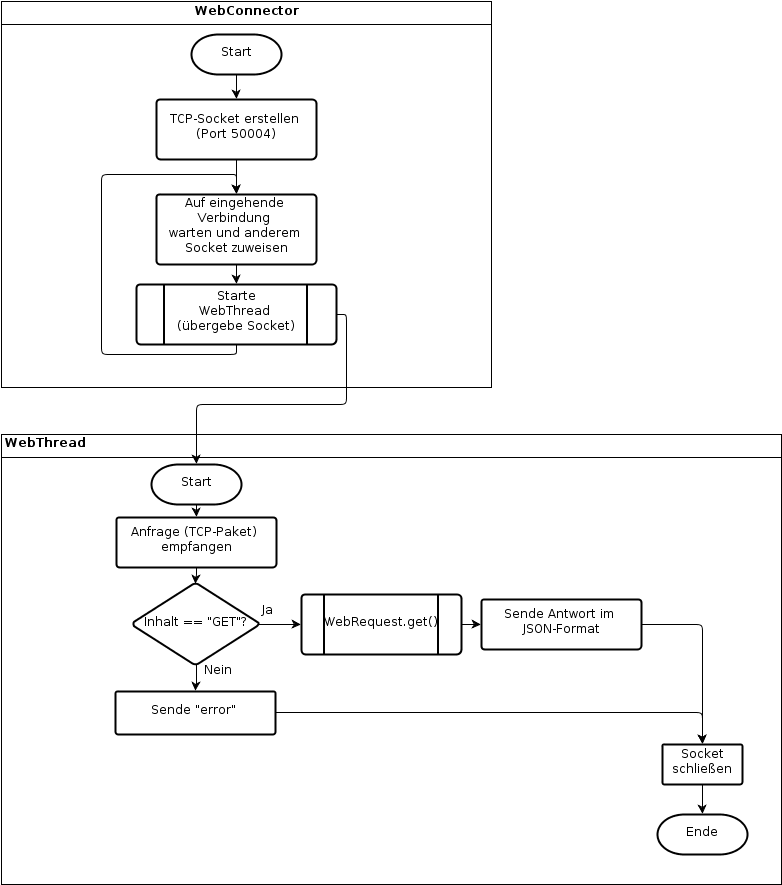
\includegraphics[width=0.63 \paperwidth]{./bilder/webConnector.png}
	\caption{WebConnector-Thread}
	\label{webconnector}
	\end{center}
	\end{minipage}
}
\end{center}
\end{figure}

\newpage
Der WebConnector-Thread wird beim Start des Daemons automatisch ausgeführt. Dabei erstellt dieser einen TCP-Socket (Port 50004), um auf eine eingehende Verbindung zu hören, die dann einem weiteren Socket zugewiesen wird. Für die weitere Bearbeitung der Anfrage wird nun ein WebThread gestartet, wobei ihm der Socket übergeben wird. Während der WebConnector jetzt wieder auf eine eigehende Verbindung wartet, führt der WebThread folgende Schritte durch:

Er empfängt die eigentliche TCP-Anfrage der Anwendung. Dabei versteht er alle Requests, die mit GET beginnen, sonst sendet er ein ``error'' zurück. Für die verstandenen Anfragen wird die bereits erwähnte Funktion get() der WebRequest-Klasse aufgerufen, die die entsprechende Antwort als JSON-Object zurückliefert, oder \textit{null} bei unbekannter GET-Anfrage. Vorausgesetzt die get() Funktion hat ein JSON-Object zurückgeliefert, wird die Antwort über die gleiche TCP-Verbindung an die Anwendung geschickt (sonst wird ``error‘‘ gesendet). Daraufhin wird der TCP-Socket geschlossen und der WebThread beendet.   

\newpage

\subsubsection*{program.main}

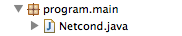
\includegraphics[width=0.24 \paperwidth]{./bilder/lib_main.png}

\begin{quote}
\begin{verbatim}
// Modulliste
public static List<Module> moduleList = 
new ArrayList<Module>();	
	
	public static void main(String[] args) {
 ...
/*1*/   UDP.sendBroadcast(Netfind.netfind(), 50000, 50001);
 ...
/*2*/   recv = UDP.receivePacket(50001, 2000);
 ...
/*3*/   module = Netfind.netdiscover(recv);
 ...
	}
\end{verbatim}
\end{quote} 

Die Klasse Netcond.java bildet den Main-Thread des Daemons, der nach dem Start zuerst ausgeführt wird. Dabei wird, wie in Abb. \ref{netcond_main} erkennbar, zunächst der WebConnector-Thread gestartet. Daraufhin folgt eine Endlosschleife, die zuerst einen UDP-Broadcast - mithilfe der bereits beschriebenen UDP-Funktionen und netfind() - von Port 50001 an Port 50000 aussendet (/*1*/) und danach in einer weiteren Endlosschleife 2 Sekunden lang auf die Antworten der Module wartet. Dazu wird wieder eine UDP-Funktion aus dem Paket lib.network benutzt (/*2*/). 

\newpage

Diese Antworten werden der Funtion netdiscover() aus dem Paket lib.protocol übergeben, die entweder ein erstelltes Objekt der Modulklasse, oder null \linebreak zurückliefert, wenn die Antwort nicht dem Protokoll entsprach (/*3*/). Wurde ein Modulobjekt zurückgegeben, wird die Modulliste - eine ArrayList die die Modulobjekte hält und in der Netcond-Klasse deklariert wurde - daraufhin dursucht, ob sie das gefunde Module bereits enthält. Ist dies nicht der Fall wird der ModuleThread des Moduls gestartet und das Modul zur Modulliste hinzugefügt. 

\begin{figure}[h]
\begin{center}
\fbox{
	%Rahmengroesse	
	\begin{minipage}{0.75 \paperwidth}
	\begin{center}
	%Bildgroesse
	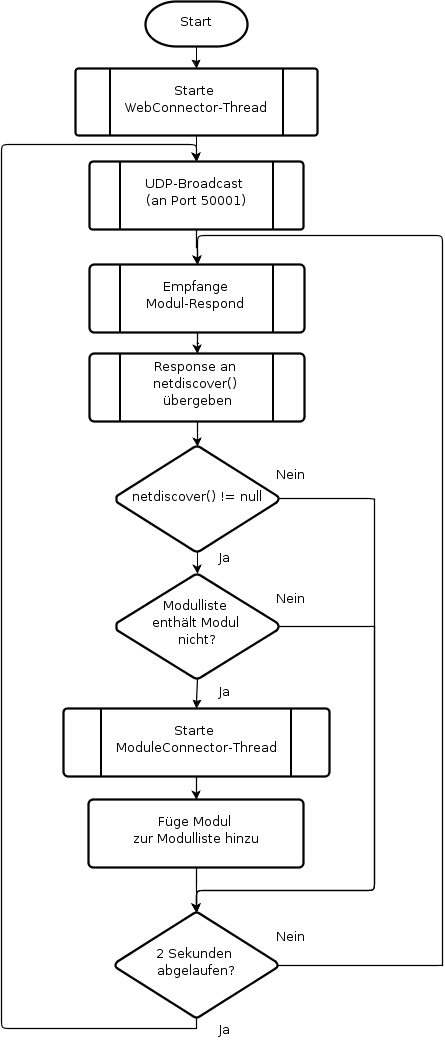
\includegraphics[width=0.30 \paperwidth]{./bilder/netcond_main.png}
	\caption{Main-Thread}
	\label{netcond_main}
	\end{center}
	\end{minipage}
}
\end{center}
\end{figure}

\newpage

\subsubsection*{Vergleich der Module}

Damit die Instanzmethode contains() der ArrayList auch feststellen kann, ob ein gefundenes Modul mit einem in der Liste enthaltenen Modul übereinstimmt, mussten die Object-Methoden equals() und hashCode() in der Klasse Module überschrieben werden. In diesem Fall stimmen zwei Module überein, wenn ihr Hostname gleich ist. 


\begin{quote}
\begin{verbatim}
@Override
public boolean equals(Object o) {
		
		Module mod = (Module) o;
		
		if (getHostname().matches(mod.getHostname()))
			return true;
		
		return false;
	}
	
@Override
	public int hashCode() {
		
		return port * super.hashCode();
	}
\end{verbatim}
\end{quote} 

\newpage
\subsubsection*{Warten im Thread}

An mehreren Stellen im Programmcode kommt es vor, dass in einem Thread gewartet werden muss. In einer Multithreading-Anwendung würde bei alleiniger Verwendung der gewohnten while-Schleife die Rechenzeit im Thread draufgehen. Stattdessen werden die Threads mit der Funktion Thread.sleep(time) schlafen gelegt und die Rechenzeit kann für die anderen Threads bzw. dem Betriebssystem genutzt werden. Um beispielsweise eine Sekunde zu warten dient folgendes Konstrukt:     

\begin{quote}
\begin{verbatim}

long startTime = System.currentTimeMillis();

while ((System.currentTimeMillis() - startTime) < 1000) {
    try {
            Thread.sleep(time);
        }	
			}

\end{verbatim}
\end{quote} 

\newpage

\subsubsection*{Synchronisation}

Greift ein Thread auf Daten zu, die auch von anderen Threads genutzt werden, muss an der Stelle im Code eine Schreibsperre für diese gesetzt werden, bis der eigene Schreibvorgang abgeschlossen ist. Auch in den Threads von netcond erfolgt ein Mehrfachschreibzugriff und zwar auf die Modulliste. Der Main-Thread fügt Module hinzu, während die einzelnen ModulThreads Daten in die Instanzvariablen der Module schreiben und auch Module löschen, am Ende ihrer Lebenszeit. Deshalb wurde jede Stelle im Programmcode, an der in die Modulliste geschrieben wird, durch ein synchronized()-Block eingehüllt.    
					
\begin{quote}
\begin{verbatim}

synchronized ( Netcond.moduleList ) {
    Netcond.moduleList.remove(module);
}

\end{verbatim}
\end{quote} 

\newpage

\subsection{netcon API}

Das \textbf{netcon Application Programming Interface (API)} ermöglicht, wie oftmals erwähnt, die Entwicklung eigener Anwendungen zur Anzeige der Moduldaten. Diese Anwendung kann beispielsweise eine Website (inkl. Webserver), oder ein Smartphone App sein. Egal wie diese auch aussehen mag, vorausgesetzt ist, dass sie die TCP-Kommunikation unterstützt. 

In diesem Abschnitt wird nun der Grundstein für die Erstellung eigener Anwendungen gelegt und das dazu notwendige API erläutert, wobei als Programmbeispiel auch die im Rahmen dieser Diplomarbeit programmierte Website herangezogen werden kann. Näheres dazu im Kapitel \textbf{Website}. 

\subsubsection*{Request}
Wurde der Daemon netcond gestartet - näheres dazu im Kapitel \textit{Installation} - wird sofort ein Thread ausgeführt, der auf Anfragen von Anwendungen wartet. Dazu muss eine TCP-Verbindung mit dem netcon-Server (an Port 50004) hergestellt werden. Schickt man nun die Anfrage, noch mit undefiniertem Inhalt an den Server, erfolgt die Konsolenausgabe \textbf{E: Incomprehensible web request} inkl. der fehlerhaften Anfrage. Damit kann schon einmal getestet werden, ob das TCP-Paket ohne Probleme beim Server ankam. 

\newpage

\subsubsection*{Response}
Der netcon Daemon sendet daraufhin die Antwort zurück an die Anwendung. Diese muss also nach dem Aussenden der Anfrage auf ein TCP-Paket warten, das die Moduldaten enthält. Wurde die Antwort empfangen, trennt der Daemon die TCP-Verbindung. Für die nächste Anfrage muss erneut eine Verbindung aufgebaut werden. 

\subsubsection*{Moduldaten empfangen}

Da zurzeit nur ein Messystem implementiert wurde, existiert auch nur ein Befehl, mit dem man eine Liste aller Module inkl. ihrer Daten erhält und zwar im JSON-Format. Dazu muss der Inhalt des TCP-Pakets folgendermaßen aussehen:

\begin{quote}
\begin{verbatim}
GET\nlist\n
\end{verbatim}
\end{quote} 

\subsubsection*{JSON}

Das Antwortpaket besteht ausschließlich aus einem leserlichen JSON-Objekt, aus dem entweder mit eigens programmierten Funktionen oder mithilfe diverser Bibliotheken die gewünschten Daten entpackt werden können. Da hier nicht auf alle verfügbaren Bibliotheken für alle Programmiersprachen eingegangen werden kann, folgt die Beschreibung des Aufbaus eines JSON-Objekts. Damit sollte es möglich sein, eigene Funktionen zu programmieren. Aber auch bei der Verwendung von bereits verfügbaren Bibliotheken empfiehlt es sich, den Aufbau zu verstehen, um die Funktionen richtig einzusetzen. 

\newpage

JSON wurde entwickelt, um den Datenaustausch zwischen Anwendungen \linebreak möglichst einfach zu gestalten und das, in einer für den Menschen gut lesbaren Form. 

Ein JSON-Objekt liegt demnach in Reintext vor, aber in genau definierter Anordnung der zu vermittelnden Daten, wobei standardmäßig die UTF-8 Kodierung verwendet wird. Es beginnt und endet mit einer geschwungenen Klammer und kann verschiedene Elemente (=Werte) enthalten, wobei jedes durch "Titel": (=Schlüssel) eingeleitet wird und mit Beistrich vom nächsten Element getrennt ist. Weiters sind Leerraum-Zeichen beliebig verwendbar.

\begin{quote}
\begin{verbatim}
{
  // Zeichenkette
    "Firmenname":"Muster Industries",
  // Boolescher Wert
    "Aktiengesellschaft":false,
  // Nullwert
    "Index":null,
  // Zahl
    "Vermögen":-150.00,
  // Array
    "Inhaber": ["Mustermann","Musterfrau"],
  // Objekt
    "Unternehmen":{
   	    "Name":"Muster Industries",
   	    "Mitarbeiterzahl": 100,
   	    "Mitarbeiter":["Adam","Eva"]
   }
}

\end{verbatim}
\end{quote}

\newpage
Wie man am Beispiel der vorherigen Seite erkennen kann, ist es sogar möglich, JSON-Objekte in sich zu verschachteln. Dieser wichtige Aspekt ist bei der Anordnung der Moduldaten zu beachten. 

Auch wichtig zu beachten ist, dass bei Verwendung von Funktionen fertiger JSON-Bibliotheken die Daten nicht in der gleichen Reihenfolge ankommen, wie sie hinzugefügt wurden. Es ist also beim Empfänger bzw. der Anwendung beim Auslesen der Daten nach dem Schlüssel zu suchen und von keiner bestimmten Reihenfolge auszugehen. Es sollte demnach immer angenommen werden, dass die Module und ihre Devices in irgendeiner Reihenfolge im JSON-Objekt vorliegen. Außerdem kann die Verwendung von Leerzeichen variieren. 

Wird nun ein TCP-Antwortpaket vom Server an die Anwendung ausgesendet, enthält es ein JSON-Objekt, das laut folgender Seite formatiert ist, wenn beispielsweise ein Modul mit zwei Devices im Netzwerk gefunden wurde. Konnte der netcon Daemon keine Module im Netzwerk finden, sieht das JSON-Objekt folgendermaßen aus: 

\begin{quote}
\begin{verbatim}
{"modulliste":null}
\end{verbatim}
\end{quote}

Wurde die Anfrage nicht verstanden, wird mit ``error'' geantwortet. 


\newpage

\begin{quote}
\begin{verbatim}
{
  "modulliste":[
    {
      "name":"AVR-NET-IO-Lipp",
      "location":"Wohnzimmer",
      "ip":"192.168.2.3",
      "port":50000,
      "uptime":"14403",
      "devicelist":[
       {"id":0,
        "type":1,
        "dtype":"f",
        "min":"0.0",
        "max":"5.0",
        "value":"0.11",
        },
        {"id":1,
        "type":1,
        "dtype":"f",
        "min":"0.0",
        "max":"5.0",
        "value":"2.0",
        }
       ]
   } //, weitere Module ...
  ]
}

\end{verbatim}
\end{quote}

\newpage

Das JSON-Objekt besteht aus einem Array, das die einzelnen Module trägt. Jedes dieser Module ist wiederum ein JSON-Objekt. Die Modulobjekte bestehen aus den Moduldaten und einem weiteren Array, das die Devices in Form von JSON-Objekten enthält. Ein Device-Objekt besteht aus seiner ID, dem Typ der Messeinheit (z.B. Volt) und des Messwerts (z.B. f für Fließkommazahl), dem minimalen und maximalen Messwert und dem Messwert. Der Typ für die Messeinheit ist in diesem Fall 1, was bedeutet, dass es sich um eine Spannung (V) handelt (von uns so festgelegt). 

Die Bedeutung der einzelnen Typen kann beliebig gewählt werden und ist im Kapitel \textit{Hardware} im Zusammenhang mit dem netcon-Protokoll, zur Kommunikation zwischen den Modulen und dem Daemon, beschrieben. Dort zu finden sind auch nähere Informationen über \textit{dtype}, den Typ des Messwerts. Diese Daten sollten reichen, um die Anzeige der Moduldaten und Messwerte (fast) unabhängig von der Messgröße zu ermöglichen. Nochmals der Hinweis, das JSON-Objekt ist in den meisten Fällen nicht so geordnet, wie die letzte Seite zeigt. Auch hier wurde im Nachhinein die Reihenfolge im Zuge der Lesbarkeit angepasst. 

Bei Problemen mit der Entwicklung eigener Anwendungen und Module ist es empfehlenswert das nächste Kapitel \textbf{Debugging} zu lesen, um diverse Fehlerquellen auszuschließen. 

\newpage

\subsection{Debugging}

\subsubsection{Ports}

Damit ein reibungsloses Zusammenspiel zwischen den Modulen und dem Daemon bzw. den Anwendungen und dem Daemon stattfinden kann, muss auf die richtige Verwendung der Ports geachtet werden. In einer Liste sind diese nocheinmal zusammengefasst. Diese sollten überprüft werden, bevor mit dem Debugging des netcon-Systems begonnen wird. Abb. \ref{kom_mod} zeigt, je nach Kommunikation, an welchen Ports die Module und Anwendungen liegen müssen bzw. von welchen Ports empfangen werden muss. Zu beachten dabei ist, dass die Ports laut Tabelle für den netcon Daemon stets frei sind und auch während der Laufzeit von keinem anderen Programm verwendet werden. Nur dann ist auch die Funktionstüchtigkeit der Software gewährleistet. Außerdem sollte darauf geachtet werden, dass der Broadcast in das richtige Netzwerk ausgesendet wird, sonst antworten die Module nicht. Dazu empfiehlt es sich, alle Netzwerkkarten zu deaktivieren die vom Daemon nicht verwendet werden. 

\begin{figure}[h]
\begin{center}
\fbox{
	%Rahmengroesse	
	\begin{minipage}{0.8 \paperwidth}
	\begin{center}
	%Bildgroesse
	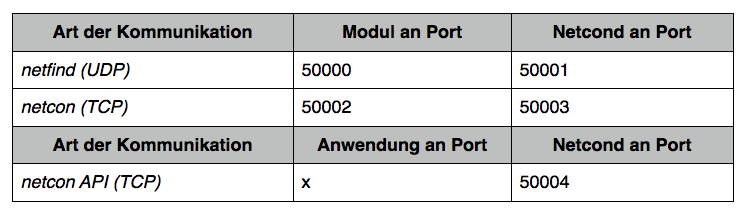
\includegraphics[width=0.7 \paperwidth]{./bilder/ports.png}
	\caption{Ports}
	\label{kom_mod}
	\end{center}
	\end{minipage}
}
\end{center}
\end{figure}

\newpage

\subsubsection{Programmausgaben}

Netcond ist, wie bereits erwähnt, eine konsolenbasierte Anwendung, die in bestimmten Fällen Textausgaben macht, um Fehler im netcon-System einfach zu entdecken:

\begin{quote}
\begin{verbatim}

I: WebConnector started

E: Incomprehensible web request (Request)

E: UDP-response isn't conform to netcon protocol (IP)

I: ModulThread started # (Hostname, IP)

E: Timeout # (Hostname, IP)

E: ModulThread stopped # (Hostname, IP)

\end{verbatim}
\end{quote} 

\textbf{I:} und \textbf{E:} geben an, ob es sich um eine Information, oder einen Fehler handelt. 

\newpage
\subsubsection*{netcon API}

Wird netcond gestartet erscheint sofort \textbf{I: WebConnector started} , nachdem der WebConnector ausgeführt wurde. Diese Information gibt Auskunft darüber, ob das netcon API bereit ist, auf Anfragen von Anwendungen zu hören. 

Schickt eine Anwendung eine nicht definierte Anfrage, erscheint \textbf{E: Incomprehensible web request} inklusive dem fehlerhaften Request.

\subsubsection*{netfind}
Antwortet ein Modul auf einen UPD-Broadcast mit einer nicht nach dem netcon-Protokoll definierten Antwort, wird  \textbf{E: UDP-response isn’t conform to netcon protocol} inklusive der IP des Moduls ausgegeben.

\subsubsection*{netcon}
Wurde ein Modul zur Modulliste hinzugefügt und der ModulThread gestartet erscheint \textbf{I: ModulThread started \#} mit Hostnamen und IP des Moduls, wobei \textbf{\#} für die Prozess-ID steht.

Antwortet das Modul beispielsweise nicht oder falsch auf die Messwertabfrage, gibt netcond \textbf{E: Timeout \# (Hostname, IP)} aus. Nach zwei misslungenen Retries erscheint dann \textbf{E: ModulThread stopped \# (Hostname, IP)} und der ModulThread wird beendet, sowie das Modul aus der Modulliste gelöscht. 

\newpage

\subsection{Website}
Informationen zur Einrichtung des Webservers für die Verwendung der Website im Kapitel \textbf{Installation}. Wird der Webserver nicht zusammen mit dem netcon Daemon auf dem selben Computer betrieben, muss eine Variable im PHP-Script angepasst werden. Näheres dazu auf den folgenden Seiten. 

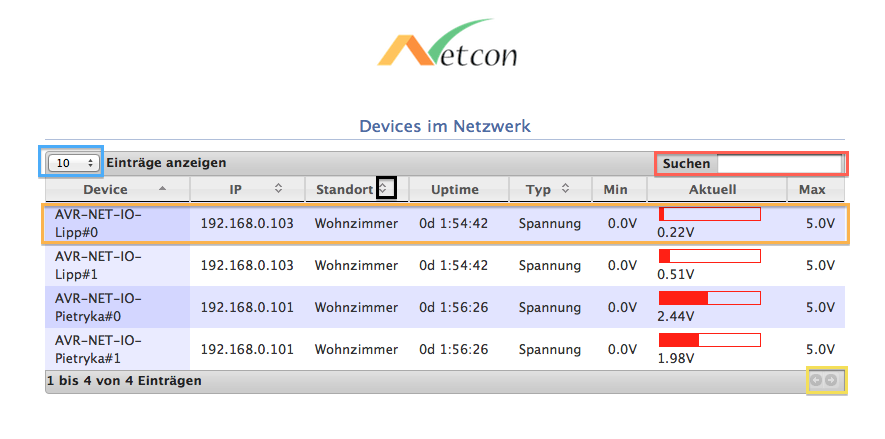
\includegraphics[width=0.85 \paperwidth]{./bilder/website2.png}

[ORANGE] Die Anzeige der Moduldaten erfolgt auf der netcon Website in einer Tabelle, wobei für jedes Device eines Moduls ein eigener Eintrag angezeigt wird. Dabei wird an den Hostnamen des Moduls einfach die Devicenummer angehängt.
 
[SCHWARZ] Standardmäßig werden die Einträge nach dem Hostnamen sortiert. Dies kann durch Drücken der entprechenden Buttons für IP, Standort und Typ verändert werden.  
 
\newpage
 
[BLAU] Mit einer Dropdown-Liste oben links kann die Anzahl der Einträge pro Seite eingestellt werden.
 
[GELB] Die Seiten können mit den Pfeiltasten unten rechts gewechselt werden.
 
[ROT] Über die Suche oben rechts kann nach allen Ausdrücken gefiltert werden z.B. Spannung oder Wohnzimmer.   
 
Kann keine Verbindung zum netcon Daemon hergestellt werden, weil dieser nicht gestartet wurde, oder die host-Variable im PHP-Script falsch gesetzt ist, sieht die Website folgendermaßen aus\footnote{Damit diese Ausgabe ordnungsgemäß erfolgt, müssen eventuell Anpassungen in den Konfigurationsdateien des Webservers durchgeführt werden. Näheres dazu im Kapitel Installation}:
 
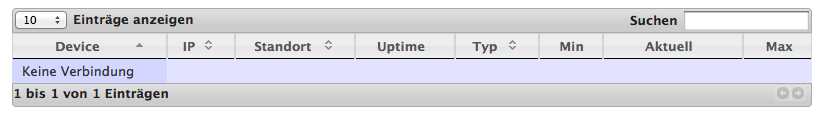
\includegraphics[width=0.85 \paperwidth]{./bilder/no_connection.png}

Wurde die Verbindung hergestellt, aber keine Module im Netzwerk gefunden, macht die Website diese Ausgabe: 

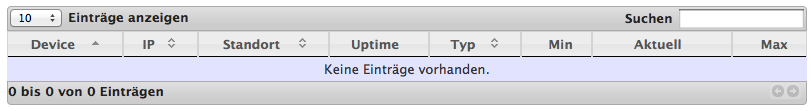
\includegraphics[width=0.85 \paperwidth]{./bilder/no_modules.png} 

\newpage

\begin{center}
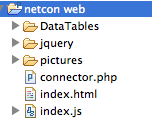
\includegraphics[width=0.20 \paperwidth]{./bilder/website_aufbau.png}
\end{center}

Die Grundlage der Website bildet das PHP-Script connector.php, das bei Aufruf den Webserver dazu veranlasst eine TCP-Anfrage an den netcon Deamon zu richten und die Moduldaten im JSON-Format entgegennimmt und ausgibt. 

Dazu wird mithilfe der PHP-Funktionen ein TCP-Socket (1) erstellt mit dem Zielport 50004. Trat kein Fehler auf, folgt nun die Anfrage GET list (2), deren Antwort daraufhin (3) eingelesen und ausgegeben (4) wird. Dieses Script liefert lediglich eine Ausgabe der Moduldaten im JSON-Format bzw. {``modulliste'':null} wenn kein Modul gefunden wurde, oder ``error''\footnote{vorausgesetzt die Anzeige von PHP-Fehlern ist deaktiviert} wenn keine Verbindung zum Daemon hergestellt werden konnte. Zur Verarbeitung und benutzerfreundlichen Anzeige sind noch weitere Schritte notwendig.  

Wichtig für die eigene Verwendung der Website ist die Anpassung der \$host-Variablen, wenn Webserver und netcon Daemon nicht gemeinsam auf einer Maschine ausgeführt werden. Ist dies der Fall, muss hier ``localhost'' durch die IP-Adresse des Webservers (unter Anführungszeichen) ersetzt werden.  

\newpage

\begin{quote}
\begin{verbatim}

    <?php
    $out = "";
    $host="localhost";
    $port=50004;
    $timeout=30;

(1) $sk=fsockopen($host,$port,$errnum,$errstr,$timeout);

    if(!is_resource($sk)) {				
        exit("error");		
    }

    else {					
(2)     fputs($sk, "GET\n", 4);
        fputs($sk, "list\n", 5);
        					
(3)     $zeichen = fgetc($sk);
    				
        while($zeichen != "\n") {
            $out .= $zeichen;
            $zeichen = fgetc($sk);
        }	
    				
(4)      echo $out;					
    }	
		
    fclose($sk);	
    ?>

\end{verbatim}
\end{quote} 

\newpage

Die eigentliche Website index.html enthält Befehle für die Einbindung von jQuery (Bibliothek mit erweiterten JavaScript-Funktionen), DataTables (Tabellen-Plugin für jQuery) und einer JavaScript-Datei, die die eigentliche Aufbereitung der Daten übernimmt. Im Body befindet sich lediglich das Logo, der Titel und eine leere Tabelle inkl. Spaltennamen, die von der DataTables-Library benötigt wird.  
 
Wurde die Website - also index.html - fertig geladen, folgt die Ausführung des JS-Scripts index.js, das sofort die Funktion \$(document).ready() ausführt, der als Paramater die Definition einer Funktion mit dem auszuführenden Programmcode übergeben wird. 

\begin{quote}
\begin{verbatim}

$(document).ready(function(){ 
    updateTable();
    window.setInterval(updateTable, 1000);
}); 

function initTable() {
    // ...
}
 
function updateTable() {
    var oTable = initTable();
    // ...
}

\end{verbatim}
\end{quote} 

\newpage

In diesem Fall ist das updateTable(), eine im selben Script definierte Funktion. Diese ruft die Funktion initTable() auf, die die Initalisierung einer leeren DataTable übernimmt und dabei ihre Formatierung festlegt (Sortierreihenfolge, Aussehen,...). Dazu nimmt sie die HTML-Tabelle als Grundgerüst, baut darauf die DataTable auf, die noch immer nur aus den Spaltennamen besteht und gibt sie an die Variable \textit{oTable} zurück. 

Danach wird das connector.php Script aufgerufen (1), die Ausgabe in einem JSON-Objekt gespeichert (3) und verarbeitet und für jedes Device ein Eintrag zur DataTable hinzugefügt (4) vorausgesetzt das JSON-Objekt enthält Module. Die Ausgabe des connector.php Scripts wird natürlich schon am Anfang darauf geprüft, ob sie ``error'' enthält (2).

\begin{quote}
\begin{verbatim}
(1)  $.get('connector.php', function(result){

(2)     if(result == "error") { 
          //...
          return;
        }
    
(3)      var json = $.parseJSON(result);
    
        // Verarbeitung ...
    
(4)      oTable.fnAddData ( [
    
          // ... 
                
        ]);
    }
\end{verbatim}
\end{quote}  
Bisher würde die Website einmal die Daten vom Daemon abfragen und in der DataTable ausgeben. Eine Methode, die den Namen Ajax trägt, macht es aber möglich die Moduldaten abzufragen, ohne die Website neu laden zu müssen. Dazu dient die zweite Zeile. Diese ruft die Funktion updateTable() jede Sekunde auf:

\begin{quote}
\begin{verbatim}
window.setInterval(updateTable, 1000);
\end{verbatim}
\end{quote}  

Zurzeit versteht die Website nur den Typ 1 (Spannung), da keine anderen Typen definiert wurden. Die Typen können in eigenen Anwendungen beliebig vergeben werden. Neue Typen können den folgenden zwei Funktionen mitgeteilt werden: 

\begin{quote}
\begin{verbatim}
function getTypeunit(typeNum) {
    switch (typeNum) {
        case 1:
            return 'V';
            break;
    }
}

function getLongType(typeNum) {
    switch (typeNum) {
        case 1:
            return 'Spannung';
            break;
    }
}
\end{verbatim}
\end{quote}  
 
\newpage

\subsection{Installation}

Der Java Daemon netcond liegt als .jar Datei vor.\footnote{/netcon Software/netcond/release/netcond.jar} Auf einem Betriebssystem mit grafischer Oberfläche könnte er einfach per Doppelklick gestartet werden, vorausgesetzt eine Java Runtime Environment in Version 6 (oder höher) ist installiert. Da es sich aber um eine konsolenbasierte Anwendung handelt, würden dann keinerlei Ausgaben sichtbar sein und der Daemon unsichtbar im Hintergrund laufen. Deshalb empfiehlt es sich, auch unter grafischen Betriebssystemen die netcond.jar Datei über die Konsole auszuführen:
\begin{quote}
\begin{verbatim}
java -jar netcond.jar
\end{verbatim}
\end{quote}

Auf Systemen ohne Monitor müsste die .jar Datei beispielsweise per SSH-Zugang übertragen und ausgeführt werden. Die Einrichtung des SSH-Zugangs für Systeme ohne Monitor wird in dieser Diplomarbeit nicht weiter behandelt, wobei der SSH-Zugang unter Linux-basierten Systemen in vielen Fällen bereits eingerichtet ist. Danach sollte mit dem Befehl ssh und der IP des Zielsystems zugegriffen werden können. 

Für die Verwendung der Beispielwebsite wird ein PHP-fähiger Webserver, wie zum Beispiel Apache, oder lighttpd (inkl. PHP-Modul) benötigt, der nicht gemeinsam mit dem netcon Deamon auf einem Computer laufen muss. Wurde der Webserver gestartet, müssen nur noch alle Dateien aus dem Verzeichnis netcon web\footnote{/netcon Software/netcon web} ind das root-Verzeichnis des Servers kopiert werden. Tippt man nun \textit{http://localhost} in die Adresszeile seines Browsers, erscheint die Website.   

\subsubsection{JRE}
Die Java Runtime Environment (JRE) ist ein Java-Interpreter, der benötigt wird um den in Bytecode vorliegenden Daemon netcond auszuführen. Sie muss in Version 6 oder höher vorliegen. 

\textbf{Windows}

Für die Installation der JRE unter Windows (XP,Vista,7,8) muss lediglich die neuste Version von \textit{http://www.java.com/de/download/} geladen und die .exe Datei installiert werden. Der java-Befehl ist danach in der Eingabeaufforderung verfügbar. 

\textbf{Mac OS X}

Alle User der neuesten Version Mac OS X Version besitzen bereits eine JRE, die womöglich noch über die Softwareaktualisierung aktualisiert werden muss.\footnote{Apple wird in naher Zukunft Java nicht mehr selbst entwickeln und aktualisieren. Die Weiterentwicklung wurde wieder an Oracle übergeben und in der nächsten Mac OS X Version wird die JRE womöglich von der Oracle-Website bezogen werden müssen.} Danach ist lediglich das Terminal zu öffnen und die .jar Datei auszuführen. 

\newpage

\textbf{Linux}

Da jede Linux-Distribution einen anderen Paketmanager verwendet um Anwendungen zu installieren/deinstallieren, hier nur eine allgemeine Erklärung. Der jeweilige Paketmanager muss gestartet und nach einem Paket mit den Inhalten ``java'' und ``oracle'' oder ``sun'' (ehemaliger Hersteller) gesucht werden. Nachdem das Paket installiert wurde, ist der java-Befehl in der Konsole verfügbar.  

Manche Distributionen, vorallem gekaufte, besitzen in vielen Fällen bereits eine JRE. Es empfiehlt sich einfach in der Konsole zu prüfen, ob der Befehl ``java'' verstsanden wird. In freien Distributionen sind oftmals proprietäre Pakete, wie java, aus lizenzrechtlichen Gründen nicht standardmäßig freigeschaltet. Um solche Pakete finden und installieren zu können, muss dies in den Einstellungen des Paketmanagers gesetzt sein.  

\newpage

\subsubsection{Webserver}
Hier wird am Beispiel von XAMPP die Installation eines PHP-fähigen Webservers erklärt. XAMPP ist ein kostenloses Programmpaket, das alle nötigen Komponenten (Apache, PHP,...) eines Webservers mitbringt und für Windows, Mac OS und Linux verfügbar ist.\footnote{http://www.apachefriends.org/de/xampp.html} Nach Installation des Webservers sollte die php.ini-Datei im xampp bzw. lampp Ordner angepasst werden, um die Anzeige von PHP-Fehlern zu unterdrücken. Nur dann erfolgt auch die im Kapitel Website erwähnte Ausgabe ``Keine Verbindung''. Dazu ist die Zeile \textit{display\_errors=On} in \textit{display\_errors=Off} zu ändern. 

\textbf{Windows}

Unter Windows ist die Installation von XAMPP genauso einfach, wie die der JRE. Von der XAMPP-Website wird die .exe-Datei geladen und per Doppelklick installiert. Danach werden die Dateien der Website nach \textit{C:\textbackslash xampp\textbackslash htdocs} kopiert und XAMPP über das Programmsymbol XAMPP Control Panel Application ausgeführt. Nun kann über den Start/Stop-Button der Webserver gestartet werden. Im Browser sollte durch Eingabe von \textit{http://localhost} die Website verfügbar sein. 

\textbf{Mac OS X}

Mac-User laden die .dmg-Datei von der XAMPP-Website und mounten diese per Doppelklick. Danach ist bloß der XAMPP-Ordner nach \textit{/Applications/} zu kopieren. Nachdem die Website in den htdocs-Ordner im Applications-Verzeichnis kopiert wurde, kann der Webserver über das Programm XAMPP Control über den Start/Stopp-Button gestartet und die Website im Browser mit \textit{http://localhost} aufgerufen werden. 

\newpage

\textbf{Linux}

Unter Linux ist für die Installation und Inbetriebnahme von XAMPP keine grafische Oberfläche notwendig. Somit steht dem Betrieb auf Embedded Systems nichts im Wege. 

Das tar.gz-Archiv muss von der XAMPP-Website heruntergeladen werden. Für die Installation werden zunächst mit dem Kommando \textit{su} root-Rechte erlangt und das Archiv mittels \textit{tar xvfz xampp-linux-1.7.7.tar.gz -C /opt} entpackt. XAMPP wurde damit ins Verzeichnis \textit{/opt} installiert. In den Ordner \linebreak \textit{/opt/lampp/htdocs} ist nun die Website zu kopieren und der Webserver mit dem Kommando \textit{/opt/lampp/lampp start} auszuführen. War der Start erfolgreich, sollte ``XAMPP gestartet'' ausgegeben werden. Verfügt das Linux-System über eine grafische Oberfläche, kann jetzt im Webbrowser mit \textit{http://localhost} die Website aufgerufen werden. Sonst verbindet man sich über einen grafischen Client (z.B. Smartphone) mit dem Webserver.

\newpage
\addcontentsline{toc}{section}{Literatur}
\section*{Literatur}
\markboth{Literatur}{Literatur}
Wikipedia. OSI-Modell.\newline
Internet: http://de.wikipedia.org/wiki/OSI-Modell, Stand: 24.05.2012

Wikipedia. Ethernet.\newline
Internet: http://de.wikipedia.org/wiki/Ethernet, Stand: 24.05.2012

Wikipedia. Internet Protocol.\newline
Internet: http://de.wikipedia.org/wiki/Internet\_Protocol, Stand: 24.05.2012

Wikipedia. User Datagram Protocol.\newline
Internet: http://tinyurl.com/6k4rmg, Stand: 24.05.2012

Wikipedia. Transmission Control Protocol\newline
Internet: http://tinyurl.com/hrchf, Stand: 24.05.2012

Adam Dunkels. The uIP Embedded TCP/IP Stack (2006)

Oracle. Java API\newline
Internet: http://docs.oracle.com/javase/6/docs/api/, Stand: 24.05.2012

Wikipedia. JavaScript Object Notation\newline
Internet: http://tinyurl.com/249jswy, Stand: 24.05.2012

jQuery. Documentation\newline
Internet: http://docs.jquery.com/Main\_Page, Stand: 24.05.2012

\newpage
php-einfach.de.\newline
http://www.php-einfach.de/, Stand: 25.05.2012

datatables.net.\newline
http://datatables.net/, Stand: 25.05.2012

w3schools.com.\newline
http://www.w3schools.com/, Stand: 25.05.2012

Atmel. ATmega32 Datasheet (2011)

Microchip. ENC28J60 Datasheet (2004)

mikrocontroller.net.\newline
http://www.mikrocontroller.net/, Stand: 25.05.2012

Silicon Labs. CP220 Datasheet (2007)

AVR Libc Documentation.\newline
http://www.nongnu.org/avr-libc/user-manual/, Stand: 24.05.2012

SDCC Compiler User Guide. (2011)

\end{document}